\def\OptimizaTikZ{2}

% Configuration file
%%%%%%%%%%%%%%%%%%%%%%%%%%%%%%%%%%%%%%%%%%%%%%%%%%%%%%%%%%%%%%%%%%%%%%%%
% Plantilla TFG/TFM
% Escuela Politécnica Superior de la Universidad de Alicante
% Realizado por: Jose Manuel Requena Plens
% Contacto: info@jmrplens.com / Telegram:@jmrplens
%%%%%%%%%%%%%%%%%%%%%%%%%%%%%%%%%%%%%%%%%%%%%%%%%%%%%%%%%%%%%%%%%%%%%%%%

%%%%%%%%%%%%%%%%%%%%%%%%
% FORMATO DEL DOCUMENTO
%%%%%%%%%%%%%%%%%%%%%%%%
% scrbook es la clase de documento
% Si se desea que no haya página en blanco entre capítulos añadir "openany" en los parámetros de la clase. Sino siempre los capítulos empezarán en página impar.
\documentclass[a4paper,11pt,titlepage]{scrbook}
\KOMAoption{toc}{bib,chapterentryfill} % Opciones del índice
\usepackage{scrhack} % Previene algunos errores
% Paquete de formato para scrbook. Con marcas, linea-separador superior e inferior
\usepackage[automark,headsepline,footsepline]{scrlayer-scrpage}
\clearpairofpagestyles		% Borra los estilos por defecto
%%
% Formato y contenido de la información de cabecera y pie de página
%%
% Información de capítulo en cabecera e interno
\ihead{{\color{gray30}\scshape\small\headmark}}	
% Número de página en cabecera y externo
\ohead{\normalfont\pagemark} 
% Número de página en pie de página y externo. Sólo en páginas sin cabecera
\ofoot[\normalfont\pagemark]{}
%% 		
% Edición del contenido de las distintas partes de la cabecera
%%
\renewcommand{\chaptermark}[1]{\markboth{#1}{}} % Capítulo (Solo texto)
\renewcommand{\sectionmark}[1]{\markright{\thesection. #1}} % Sección (Número y texto)
\setkomafont{pagenumber}{} % Número de página (Sin nada añadido)

% Añade al índice y numera hasta la profundidad 4.
% 1:section,2:subsection,3:subsubsection,4:paragraph
\setcounter{tocdepth}{4}
\setcounter{secnumdepth}{4}
% Muestra una regla para comprobar el formato de las páginas
%\usepackage[type=upperleft,showframe,marklength=8mm]{fgruler}
% MÁRGENES DE LAS PÁGINAS
\usepackage[
  inner	=	3.0cm, % Margen interior
  outer	=	2.5cm, % Margen exterior
  top	=	2.5cm, % Margen superior
  bottom=	2.5cm, % Margen inferior
  includeheadfoot, % Incluye cabecera y pie de página en los márgenes
]{geometry}
% Valor de interlineado
\renewcommand{\baselinestretch}{1.0} % 1 línea de interlineado
% Para poder generar páginas horizontales
\usepackage{lscape}
% Ancho de la zona para comentarios en el margen. (modificado para todonotes)
\setlength{\marginparwidth}{1.9cm}

%%%%%%%%%%%%%%%%%%%%%%%%
% BIBLIOGRAFÍA
%%%%%%%%%%%%%%%%%%%%%%%%
\usepackage{apacite} % NORMA APA
\usepackage{natbib}
\usepackage{breakcites}

%%%%%%%%%%%%%%%%%%%%%%%%
% DOCUMENTO EN ESPAÑOL
%%%%%%%%%%%%%%%%%%%%%%%%
\usepackage[base]{babel}
\usepackage{polyglossia}
\setdefaultlanguage{english}

% \addto\captionsspanish{%
% 	\renewcommand{\listtablename}{List of Tables} 
% 	\renewcommand{\tablename}{Table}
% 	\renewcommand{\lstlistingname}{Code}
% 	\renewcommand{\lstlistlistingname}{List of \lstlistingname s}
% 	\renewcommand{\glossaryname}{Glossary}
% 	\renewcommand{\acronymname}{Acronyms}
% 	\renewcommand{\bibname}{Bibliography}%
% }

%%%%%%%%%%%%%%%%%%%%%%%% 
% COLORES
%%%%%%%%%%%%%%%%%%%%%%%% 
% Biblioteca de colores
\usepackage{color}
\usepackage[dvipsnames]{xcolor}
% Otros colores definidos por el usuario
\definecolor{gray97}{gray}{.97}
\definecolor{gray75}{gray}{.75}
\definecolor{gray45}{gray}{.45}
\definecolor{gray30}{gray}{.30}
\definecolor{negro}{RGB}{0,0,0}
\definecolor{blanco}{RGB}{255,255,255}
\definecolor{dkgreen}{rgb}{0,.6,0}
\definecolor{dkblue}{rgb}{0,0,.6}
\definecolor{dkyellow}{cmyk}{0,0,.8,.3}
\definecolor{gray}{rgb}{0.5,0.5,0.5}
\definecolor{mauve}{rgb}{0.58,0,0.82}
\definecolor{deepblue}{rgb}{0,0,0.5}
\definecolor{deepred}{rgb}{0.6,0,0}
\definecolor{deepgreen}{rgb}{0,0.5,0}
\definecolor{MyDarkGreen}{rgb}{0.0,0.4,0.0}
\definecolor{bluekeywords}{rgb}{0.13,0.13,1}
\definecolor{greencomments}{rgb}{0,0.5,0}
\definecolor{redstrings}{rgb}{0.9,0,0}

%%%%%%%%%%%%%%%%%%%%%%%%
% TABLAS
%%%%%%%%%%%%%%%%%%%%%%%%
% Paquetes para tablas
\usepackage{longtable,booktabs,array,multirow,multicol,tabularx,ragged2e,array}
% Nuevos tipos de columna para tabla, se pueden utilizar como por ejemplo C{3cm} en la definición de columnas de la función tabular
\newcolumntype{L}[1]{>{\raggedright\let\newline\\\arraybackslash\hspace{0pt}}m{#1}}
\newcolumntype{C}[1]{>{\centering\let\newline\\\arraybackslash\hspace{0pt}}m{#1}}
\newcolumntype{R}[1]{>{\raggedleft\let\newline\\\arraybackslash\hspace{0pt}}m{#1}}

%%%%%%%%%%%%%%%%%%%%%%%% 
% GRAFICAS y DIAGRAMAS 
%%%%%%%%%%%%%%%%%%%%%%%% 
% Paquete para todo tipo de gráficas, diagramas, modificación de imágenes, etc
\usepackage{tikz,tikzpagenodes}
\usetikzlibrary{tikzmark,calc,shapes.geometric,arrows,backgrounds,shadings,shapes.arrows,shapes.symbols,shadows,positioning,fit,automata,patterns,intersections}
\usepackage{pgfplots}
\pgfplotsset{colormap/jet}
\pgfplotsset{compat=newest} % Compatibilidad
\usepgfplotslibrary{patchplots,groupplots,fillbetween,polar}
\usepackage{pgfplotstable}
% Guardar las figuras realizadas con Tikz y Pgf en una carpeta externa
% para agilizar el procesado y tenerlas para utilizarlas en otros
% documentos
\if\OptimizaTikZ 1
\usepgfplotslibrary{external}
\tikzexternalize[prefix=images/] % Ruta
\tikzset{%
    external/system call ={xelatex -enable-write18 -halt-on-error -interaction=batchmode -jobname "\image" "\texsource"},
}
\fi

% Estilos para elementos graficos
% Cajas y cajas de texto
\tikzstyle{Caja1} = [green,very thick,rounded corners,fill=white, fill opacity=0.5]
\tikzstyle{Texto1} = [fill=white,thick,shape=circle,draw=black,inner sep=2pt,font=\sffamily,text=black]
\tikzstyle{Texto2} = [fill=white,thick,shape=rectangle,draw=black,inner sep=2pt,font=\sffamily,text=black]
\tikzstyle{Texto3} = [fill=white,thick,shape=circle,draw=black,inner sep=2pt,font=\sffamily,text=black]
% Cuadros de diagrama
\tikzstyle{rectvioleta} = [rectangle, rounded corners, text centered, draw=black, fill=blue!10]
\tikzstyle{rectnaranja} = [rectangle, minimum width=2cm, minimum height=1cm, text centered, draw=black, fill=orange!10]
\tikzstyle{romborosa} = [diamond, aspect=3, minimum width=3cm, minimum height=1cm, text centered, draw=black, fill=red!10]
\tikzstyle{rectverde} = [rectangle, minimum width=2cm, minimum height=1cm, text centered, draw=black, fill=green!10]
\tikzstyle{rectamarillo} = [rectangle, rounded corners, minimum width=2cm, minimum height=1cm, text centered, draw=black, fill=yellow!10]
% Flechas
\tikzstyle{arrow} = [thick,->,>=stealth]

%%%%%%%%%%%%%%%%%%%%%%%% 
% FIGURAS, TABLAS, ETC 
%%%%%%%%%%%%%%%%%%%%%%%% 
\usepackage{subcaption} % Para poder realizar subfiguras
\usepackage{caption} % Para aumentar las opciones de diseño
% Nombres de figuras, tablas, etc, en negrita la numeración, todo con letra small
\captionsetup{labelfont={bf,small},textfont=small}
% Paquete para modificar los espacios arriba y abajo de una figura o tabla
\usepackage{setspace}
% Define el espacio tanto arriba como abajo de las figuras, tablas
\setlength{\intextsep}{5mm}
% Para ajustar tamaños de texto de toda una tabla o grafica
% Uso: {\scalefont{0.8} \begin{...} \end{...} }
\usepackage{scalefnt}
% Redefine las tablas y figuras para eliminar el '.' entre la numeración y el texto
\renewcommand*{\figureformat}{\figurename~\thefigure}
\renewcommand*{\tableformat}{\tablename~\thetable}

%%%%%%%%%%%%%%%%%%%%%%%% 
% TEXTO
%%%%%%%%%%%%%%%%%%%%%%%%
% Paquete para poder modificar las fuente de texto
\usepackage{xltxtra}
% Cualquier tamaño de texto. Uso: {\fontsize{100pt}{120pt}\selectfont tutexto}
\usepackage{anyfontsize}
% Para modificar parametros del texto.
\usepackage{setspace}
% Paquete para posicionar bloques de texto
\usepackage{textpos}
% Paquete para realizar cajas de texto. 
% Uso: \begin{mdframed}[linecolor=red!100!black] tutexto \end{mdframed}
\usepackage{framed,mdframed}
% Para subrayar. Uso: \hlc[tucolor]{tutexto}
\newcommand{\hlc}[2][yellow]{ {\sethlcolor{#1} \hl{#2}} }

%%%%%%%%%%%%%%%%%%%%%%%% 
% OTROS
%%%%%%%%%%%%%%%%%%%%%%%%
% Para hacer una pagina horizontal. Uso: \begin{landscape} xxxx \end{lanscape}
\usepackage{lscape} 
% Para incluir paginas PDF. Uso:
% \includepdf[pages={1}]{tuarchivo.pdf}
\usepackage{pdfpages}
% Para introducir url's con formato. Uso: \url{http://www.google.es}
\usepackage{url}
% Amplia muchas funciones graficas de latex
\usepackage{graphicx}
% Paquete que añade el hipervinculo en referencias dentro del documento, indice, etc
% Se define sin bordes alrededor. Uso: \ref{tulabel}
\usepackage[pdfborder={000}]{hyperref}
\usepackage{float}
\usepackage{placeins}
\usepackage{afterpage}
\usepackage{verbatim}
% Paquete para condicionales avanzados
\usepackage{xstring,xifthen}
% Paquete para realizar calculos en el código
\usepackage{calc}
% Para rotar tablas o figuras o su contenido
\usepackage{rotating} 
% Para incluir comentarios en el texto. El parámetro 'disable' oculta todas las notas.
% USO: \todo{tutexto}
\usepackage[textsize=tiny,shadow,textwidth=2cm]{todonotes}
%\reversemarginpar % Descomentar si se quiere todos los comentarios en el mismo lado
% Desactiva la exportación de los ToDo y Missingfigures como figuras
\if\OptimizaTikZ 1
\makeatletter
\renewcommand{\todo}[2][]{\tikzexternaldisable\@todo[#1]{#2}\tikzexternalenable}
\makeatother
\usepackage{letltxmacro}
\LetLtxMacro{\oldmissingfigure}{\missingfigure}
\makeatletter
\renewcommand{\missingfigure}[2][]{\tikzexternaldisable\oldmissingfigure[{#1}]{#2}\tikzexternalenable}
\makeatother
\fi

%%%%%%%%%%%%%%%%%%%%%%%% 
% GLOSARIOS
%%%%%%%%%%%%%%%%%%%%%%%%
\usepackage[acronym,nonumberlist,toc]{glossaries}
\usepackage{glossary-superragged}
\newglossarystyle{modsuper}{%
  \setglossarystyle{super}%
  \renewcommand{\glsgroupskip}{}
}
\renewcommand{\glsnamefont}[1]{\textbf{#1}}


%%%%%%%%%%%%%%%%%%%%%%%% 
% COMANDOS AÑADIDOS
%%%%%%%%%%%%%%%%%%%%%%%%
% Para mostrar la fecha actual (mes año) con \Hoy
\newcommand{\MONTH}{%
  \ifcase\month% 0
    \or January% 1
    \or February% 2
    \or March% 3
    \or April% 4
    \or May% 5
    \or June% 6
    \or July% 7
    \or August% 8
    \or September% 9
    \or October% 10
    \or November% 11
    \or December% 12
  \fi}
\newcommand{\YEAR}{\number\year}
\newcommand{\Today}{\MONTH\ \YEAR}

%%%%%%%%%%%%%%%%%%%%%%%% 
% MATEMÁTICAS
%%%%%%%%%%%%%%%%%%%%%%%%
\usepackage{mathtools,amsthm,amsfonts,amssymb,bm,mathrsfs,nicefrac,upgreek,bigints} 
% Comando para añadir información de variables a las ecuaciones
% Uso: \begin{condiciones}[donde:] ....... \end{condiciones}
\newenvironment{conditionals}[1][2]
  {%
   #1\tabularx{\textwidth-\widthof{#1}}[t]{
     >{$}l<{$} @{}>{${}}c<{{}$}@{} >{\raggedright\arraybackslash}X
   }%
  }
  {\endtabularx\\[\belowdisplayskip]}

%%%%%
% PARÁMETROS DE FORMATO DE CODIGOS
%%%%%
% Puedes editar los formatos para ajustarlos a tu gusto
%%%%%%%%%%%%%%%%%%%%%%%%%%%%%%%%%%%%%%%%%%%%%%%%%%%%%%%%%%%%%%%%%%%%%%%%
% Plantilla TFG/TFM
% Escuela Politécnica Superior de la Universidad de Alicante
% Realizado por: Jose Manuel Requena Plens
% Contacto: info@jmrplens.com / Telegram:@jmrplens
%%%%%%%%%%%%%%%%%%%%%%%%%%%%%%%%%%%%%%%%%%%%%%%%%%%%%%%%%%%%%%%%%%%%%%%%


%%%%%%%%%%%%%%%%%%%%%%%% 
% CÓDIGO. CONFIGURACIÓN. En el siguiente bloque están los estilos.
%%%%%%%%%%%%%%%%%%%%%%%%
% Paquete para mostrar código de matlab. En caja y lineas numeradas
\usepackage[framed,numbered]{matlab-prettifier}
% Paquete mostrar código de programación de distintos lenguajes
\usepackage{listings}
\lstset{ inputencoding=utf8,
extendedchars=true,
frame=single, % Caja donde se ubica el código
backgroundcolor=\color{gray97}, % Color del fondo de la caja
rulesepcolor=\color{black},
boxpos=c,
abovecaptionskip=-4pt,
aboveskip=12pt,
belowskip=0pt,
lineskip=0pt,
framerule=0pt,
framextopmargin=4pt,
framexbottommargin=4pt,
framexleftmargin=11pt,
framexrightmargin=0pt,
linewidth=\linewidth,
xleftmargin=\parindent,
framesep=0pt,
rulesep=.4pt,
stringstyle=\ttfamily,
showstringspaces = false,
showspaces = false,
showtabs = false,
columns=fullflexible,
basicstyle=\small\ttfamily,
commentstyle=\color{gray45},
keywordstyle=\bfseries,
tabsize=4,
numbers=left,
numbersep=1pt,
numberstyle=\tiny\ttfamily\color{gray75},
numberfirstline = false,
breaklines=true,
postbreak=\mbox{\textcolor{red}{$\hookrightarrow$}\space}, % Flecha al saltar de linea
prebreak=\mbox{\textcolor{red}{$\hookleftarrow$}\space}, % Flecha al saltar de linea
literate=
  {á}{{\'a}}1 {é}{{\'e}}1 {í}{{\'i}}1 {ó}{{\'o}}1 {ú}{{\'u}}1
  {Á}{{\'A}}1 {É}{{\'E}}1 {Í}{{\'I}}1 {Ó}{{\'O}}1 {Ú}{{\'U}}1
  {à}{{\`a}}1 {è}{{\`e}}1 {ì}{{\`i}}1 {ò}{{\`o}}1 {ù}{{\`u}}1
  {À}{{\`A}}1 {È}{{\'E}}1 {Ì}{{\`I}}1 {Ò}{{\`O}}1 {Ù}{{\`U}}1
  {ä}{{\"a}}1 {ë}{{\"e}}1 {ï}{{\"i}}1 {ö}{{\"o}}1 {ü}{{\"u}}1
  {Ä}{{\"A}}1 {Ë}{{\"E}}1 {Ï}{{\"I}}1 {Ö}{{\"O}}1 {Ü}{{\"U}}1
  {â}{{\^a}}1 {ê}{{\^e}}1 {î}{{\^i}}1 {ô}{{\^o}}1 {û}{{\^u}}1
  {Â}{{\^A}}1 {Ê}{{\^E}}1 {Î}{{\^I}}1 {Ô}{{\^O}}1 {Û}{{\^U}}1
  {œ}{{\oe}}1 {Œ}{{\OE}}1 {æ}{{\ae}}1 {Æ}{{\AE}}1 {ß}{{\ss}}1
  {ű}{{\H{u}}}1 {Ű}{{\H{U}}}1 {ő}{{\H{o}}}1 {Ő}{{\H{O}}}1
  {ç}{{\c c}}1 {Ç}{{\c C}}1 {ø}{{\o}}1 {å}{{\r a}}1 {Å}{{\r A}}1
  {€}{{\euro}}1 {£}{{\pounds}}1 {«}{{\guillemotleft}}1
  {»}{{\guillemotright}}1 {ñ}{{\~n}}1 {Ñ}{{\~N}}1 {¿}{{?`}}1,
  }

% Intenta no dividir los códigos en diferentes paginas si es posible
\lstnewenvironment{listing}[1][]
   {\lstset{#1}\pagebreak[0]}{\pagebreak[0]}

% Formato de títulos de los códigos
\DeclareCaptionFont{white}{\color{white}}
\DeclareCaptionFormat{listing}{\colorbox{gray}{\parbox{\textwidth - 2\fboxsep}{#1#2#3}}}
\captionsetup[lstlisting]{format=listing,labelfont=white,textfont=white,font= scriptsize}


%%%%%%%%%%%%%%%%%%%%%%%% 
% CÓDIGO. ESTILOS. Ajústalos a tu gusto
%%%%%%%%%%%%%%%%%%%%%%%%
\lstdefinestyle{Consola}
	{
	basicstyle=\scriptsize\bf\ttfamily,
	}
   
\lstdefinestyle{C}
	{
	basicstyle=\scriptsize,
	language=C,
	}
\lstdefinestyle{C-color}
	{
  	breaklines=true,
  	language=C,
  	basicstyle=\scriptsize,
  	keywordstyle=\bfseries\color{green!40!black},
  	commentstyle=\itshape\color{purple!40!black},
  	identifierstyle=\color{blue},
  	stringstyle=\color{orange},
    }
\lstdefinestyle{CSharp}
	{
	basicstyle=\scriptsize
	language=[Sharp]C,
	escapeinside={(*@}{@*)},
	keywordstyle=\bfseries,
	}
\lstdefinestyle{CSharp-color}
	{
	basicstyle=\scriptsize
	language=[Sharp]C,
	escapeinside={(*@}{@*)},
	commentstyle=\color{greencomments},
	keywordstyle=\color{bluekeywords}\bfseries,
	stringstyle=\color{redstrings},
	}
\lstdefinestyle{C++}
	{
	basicstyle=\scriptsize,
	language=C++,
 	}
 	
\lstdefinestyle{C++-color}
	{
  	breaklines=true,
  	language=C++,
  	basicstyle=\scriptsize,
  	keywordstyle=\bfseries\color{green!40!black},
  	commentstyle=\itshape\color{purple!40!black},
  	identifierstyle=\color{blue},
  	stringstyle=\color{orange},
    }
    
\lstdefinestyle{PHP}
	{
	basicstyle=\scriptsize,
	language=PHP,
	}
	
\lstdefinestyle{PHP-color}
	{
	basicstyle=\scriptsize,
	language=PHP,
	keywordstyle    = \color{dkblue},
  	stringstyle     = \color{red},
  	identifierstyle = \color{dkgreen},
  	commentstyle    = \color{gray},
  	emph            =[1]{php},
  	emphstyle       =[1]\color{black},
  	emph            =[2]{if,and,or,else},
  	emphstyle       =[2]\color{dkyellow}
  }
  
\lstdefinestyle{Matlab}
	{
	basicstyle=\scriptsize,
	language=Matlab,
	numberstyle=\tiny\ttfamily\color{gray75},
	}
	
\lstdefinestyle{Matlab-color}
	{
	style = Matlab-editor,
	basicstyle=\scriptsize,
	numberstyle=\tiny\ttfamily\color{gray75},
	}
	
\lstdefinestyle{Latex}
	{
	language=[LaTeX]{Tex},
    basicstyle=\scriptsize,
    literate={\$}{{{\bfseries\$}}}1,
    alsoletter={\\,*,\&},
    emph =[1]{\\begin,\\end,\\caption,\\label,\\centering,\\FloatBarrier,
              \\lstinputlisting,\\scalefont,\\addplot,\\input,
              \\legend,\\item,\\subitem,\\includegraphics,\\textwidth,
              \\section,\\subsection,\\subsubsection,\\paragraph,
              \\cite,\\citet,\\citep,\\gls,\\bibliographystyle,\\url,
              \\citet*,\\citep*,\\todo,\\missingfigure,\\footnote},
  	emphstyle =[1]\bfseries,
  	emph = [2]{equation,subequations,eqnarray,figure,subfigure,
  			   condiciones,flalign,tikzpicture,axis,lstlisting,
  			   itemize,description
  			   },
  	emphstyle =[2]\bfseries,
    numbers=none,
	}
	
\lstdefinestyle{Latex-color}
	{
	language=[LaTeX]{Tex},
    basicstyle=\scriptsize,
    commentstyle=\color{dkgreen},
    identifierstyle=\color{black},
    literate={\$}{{{\bfseries\color{Dandelion}\$}}}1, % Colorea el simbolo dollar
    alsoletter={\\,*,\&},
    emph =[1]{\\begin,\\end,\\caption,\\label,\\centering,\\FloatBarrier,
              \\lstinputlisting,\\scalefont,\\addplot,\\input,
              \\legend,\\item,\\subitem,\\includegraphics,\\textwidth,
              \\section,\\subsection,\\subsubsection,\\paragraph,
              \\cite,\\citet,\\citep,\\gls,\\bibliographystyle,\\url,
              \\citet*,\\citep*,\\todo,\\missingfigure,\\footnote},
  	emphstyle =[1]\bfseries\color{RoyalBlue},
  	emph = [2]{equation,subequations,eqnarray,figure,subfigure,
  			   condiciones,flalign,tikzpicture,axis,lstlisting,
  			   itemize,description
  			   },
  	emphstyle =[2]\bfseries,
    numbers=none,
	}
\lstdefinestyle{Java}
{
	basicstyle=\scriptsize,
	language=Java,
}

\lstdefinestyle{Java-color}
{
	basicstyle=\scriptsize,
	language=Java,
  	keywordstyle=\color{blue},
  	commentstyle=\color{dkgreen},
  	stringstyle=\color{mauve},
}
\lstdefinestyle{Python}
{
	language=Python,
	basicstyle=\scriptsize,
	otherkeywords={self},  
	keywordstyle=\bfseries,     
	emphstyle=\bfseries,    
	emph={MyClass,__init__},         
}

\lstdefinestyle{Python-color}
{
	language=Python,
	basicstyle=\scriptsize,
	otherkeywords={self},          
	keywordstyle=\bfseries\color{deepblue},
	emph={MyClass,__init__},         
	emphstyle=\bfseries\color{deepred},    
	stringstyle=\color{deepgreen},
}
\lstdefinestyle{R}
{
	language=R,                     
  	basicstyle=\scriptsize,
  	keywordstyle=\bfseries, 
}
\lstdefinestyle{R-color}
{
	language=R,                     
  	basicstyle=\scriptsize,
  	keywordstyle=\bfseries\color{RoyalBlue}, 
  	commentstyle=\color{YellowGreen},
  	stringstyle=\color{ForestGreen}  
}


%%%%%
% DEFINICION DE CONCEPTOS
%%%%
% Uso ejemplo: \begin{ejemplo} tucontenido \end{ejemplo} 
\newtheorem{theorem}{Theorem}[chapter]
\newtheorem{example}{Example}[chapter]
\newtheorem{definition}{Definition}[chapter]



\newcommand{\thesisTitle}{Evolutionary Robotics}
\newcommand{\thesisSubtitle}{Beyond the transferability gap}

\newcommand{\name}{Richard Banyi}
\newcommand{\email}{riba@itu.dk}

\newcommand{\supervisorOne}{Andres Faina}
\newcommand{\supervisorSecond}{David Kadish}
\newcommand{\departamentSupervisorOne}{Robotics, Evolution, and Art Lab}
\newcommand{\departamentSupervisorSecond}{Robotics, Evolution, and Art Lab}

\newcommand{\logoITU}{include/images/itu_logo}
\newcommand{\programme}{Master of Science in Computer Science}

\hypersetup{
pdfauthor = {\name~(\email)},
pdftitle = {\thesisTitle},
}

\begin{document}

\frontmatter

%%%%%%%%%%%%%%%%%%%%%%%%%%%%%%%%%%%%%%%%%%%%%%%%%%%%%%%%%%%%%%%%%%%%%%%%
% Official Author: Jose Manuel Requena Plens
% Edited: Richard Banyi
%%%%%%%%%%%%%%%%%%%%%%%%%%%%%%%%%%%%%%%%%%%%%%%%%%%%%%%%%%%%%%%%%%%%%%%%

\begin{titlepage}

% Margins of this page modified
\newgeometry{ignoreall,top=2cm,bottom=2cm}
\newlength{\centeroffset}
% Horizontal offset for the entire cover
\setlength{\centeroffset}{-0.5\oddsidemargin}
\addtolength{\centeroffset}{0.5\evensidemargin}
\thispagestyle{empty}

% Title and subtitle
\noindent\hspace*{\centeroffset}\begin{minipage}{\textwidth}
\centering
\begin{spacing}{1.5}{\huge\bfseries \thesisTitle}\end{spacing}
\noindent\rule[-1ex]{\textwidth}{3pt}\\[3.5ex] % Linea
{\large\bfseries \thesisSubtitle\\[4cm]}
\end{minipage}

% Filling up to the central area
\vspace{2.5cm}

% Central zone. Author and Tutors
\noindent\hspace*{\centeroffset}
\begin{minipage}{\textwidth}
\centering

\textbf{Author}\\ {\name}\\[2.5ex]
\textbf{Supervisors}\\
{\normalsize \supervisorOne\\
\ifx\departamentSupervisorOne\undefined \else \small\textit \departamentSupervisorOne\\ \fi
\ifx\supervisorSecond\undefined \else \normalsize \supervisorSecond\\ \fi
\ifx\departamentSupervisorSecond\undefined \else\small\textit \departamentSupervisorSecond\\[2cm] \fi
}
\end{minipage}

% Filling up the area below
\vspace*{\fill}

\noindent\hspace*{\centeroffset}
\begin{minipage}{\textwidth}
\centering
\noindent\hspace*{\centeroffset}
\begin{center}
{\includegraphics[width=3cm]{\logoITU}}\\
{\raggedleft\programme}
\end{center}
\vspace*{2em}
\centering
\noindent\hspace*{\centeroffset}
\\[1cm]
Copenhagen, \Today
\end{minipage}

\end{titlepage}

% From here, apply the margins established in initial configuration.tex
\restoregeometry




\tableofcontents
\listoffigures
\listoftables
% \lstlistoflistings

\mainmatter

\cleardoublepage %salta a nueva página impar
\chapter*{Abstact}

\thispagestyle{empty}
\vspace{1cm}

Lorem ipsum dolor sit amet, consectetur adipiscing elit, sed do eiusmod tempor incididunt ut labore et dolore magna aliqua. Ut enim ad minim veniam, quis nostrud exercitation ullamco laboris nisi ut aliquip ex ea commodo consequat. Duis aute irure dolor in reprehenderit in voluptate velit esse cillum dolore eu fugiat nulla pariatur. Excepteur sint occaecat cupidatat non proident, sunt in culpa qui officia deserunt mollit anim id est laborum.
\chapter{Introduction}

Evolutionary Robotics concerns with the use of Evolutionary Algorithms in robotics. The use of EA in robotics is motivated by a number of issues \cite{meyer1998evolutionary} \cite{grefenstette1994evolutionary}. One of the issues is concerned with the difficulties of hard-coding the control architecture of a robot that has to solve a given task in an unknown or possible changing environment. Because it's impossible to predict each problem that a robot might encounter in a constantly changing environment. More precisely, it's difficult to program a robot control system that can foresee every possible state of its environment and the action it should take.  Another issue is related to simulation models. Building pre-defined abstract models of the world is not sufficient in a continuously changing environment since these models often fail to reflect the complexities of the real world, such as light, gravity, noise, and errors in real sensors, actuators, etc. In response to such difficulties, researchers advocate the use of EA for the development of robots that can adapt and evolve behaviors based on specific environment and problems it's facing.

Evolutionary algorithms are indeed attractive optimization procedures to apply, that merely rewards each evaluated solution with a value that reflects its performance based on a fitness function. However, this procedure often requires a large number of evaluations before optimal solutions are found. As ER concerns robots, it should theoretically be evaluated on physical robot \cite{floreano1998evolutionary}. In practice, the optimization process on a physical robot can be very time-consuming. As a result, works that apply the optimization directly on the physical robot often evaluate few individuals along with a few generations, which reduces the competence of the evolutionary methods. For instance in \cite{faina2017automating}, controllers for a small tracked robot \textit{Pololu Zumo 32U4} \footnote{Pololu. Pololu Zumo 32u4 robot, 2016. \url{https://www.pololu.com/category/170/zumo-32u4-robot}} have been evolved with a population of 15 individuals during 20 generations and 2 simulations run, that is 600 evaluations during the entire optimization process. Adding to that the time of the actual evaluation of each controller resulted in 48 hours of running time.

For this reason, simulators in ER are often an appealing way to speed up the optimization process. Accurate simulation models are designed in order to evaluate the fitness in a fully virtual set-up. Accurate simulation models are designed in order to evaluate the fitness in a fully virtual set-up. Even though accurate models are build that corresponds to reality and successful controllers are evolved, the results are often sealed in the simulated world because of inaccuracies of the simulator or bad modeled of physical features in the simulator like friction, light, aerodynamics, etc. This transfer phenomenon is called \textit{reality gap}. Reality gap remains a critical issue that prevents the use of ER for practical applications in robotics. With my thesis I want to explore/compare state-of-the-art approaches to the \textit{reality gap} problem. In particular, the focus is on three main approaches:

\begin{enumerate}
    \item Reality-based optimization process where the entire optimization takes place fully on the physical robot.
    \item Simulation-based optimization process with the entire optimization in simulation.
    \item Robot in the loop optimization process, that optimize solutions in simulation but allows transfer experiments during the evolutionary process.
\end{enumerate}

Our first essential focus is on the robot in the loop optimization process, concretely the \textit{transferability approach} \cite{koos2012transferability} which is currently the best state-of-the-art approach to bypass the reality gap. However, instead of attempting to conduct as few transfers as possible, the \textit{transferability measure} is obtained for N solutions in every generation. We hypothesize that if the \textit{surrogate model} is more accurate and updated more frequently, this would allow boosting the evolutionary search. Another insight is concerned with an accurate simulation model, which is designed to accurately mimic the dynamics of the physical environment. Optimal solutions that emerge in simulation should transfer well onto the physical robot and achieve good performance/behavior in reality. In order to quantify how well a controller evolved in simulation transfer to reality, we define a \textit{transferable measure} which compares the corresponding real and simulated behavior.

Additionally, our Evolutionary strategy consists of two approaches. The first one is concerned with evolving weights of a feedforward neural network. In the second approach, instead of evolving just the weights of ANN controllers with a fixed structure we are also optimizing ANN controllers using NEAT \cite{stanley2002evolving}. A genetic algorithm for evolving both weights and topology of artificial neural networks.

All of the above approaches will be systematically compared and validated to on a robotic application, particularly obstacle avoidance task. As we need to evaluate a lot of controllers in the real world, which is time-consuming, we build an automated robotic platform which enables us to test and validate as many transfers as we want and run the entire optimization process on the physical robot without human intervention while taking the entire physical environment into account. Likewise, a simulation model will be designed from scratch that properly describes the dynamics of the real environment.

\section{Evolutionary Algorithms and Neuroevolution}

\section{The Reality Gap}

\section{The Transferability Approach}
\chapter{Experimental Design}

Lorem ipsum dolor sit amet, consectetur adipiscing elit, sed do eiusmod tempor incididunt ut labore et dolore magna aliqua. Ut enim ad minim veniam, quis nostrud exercitation ullamco laboris nisi ut aliquip ex ea commodo consequat. Duis aute irure dolor in reprehenderit in voluptate velit esse cillum dolore eu fugiat nulla pariatur. Excepteur sint occaecat cupidatat non proident, sunt in culpa qui officia deserunt mollit anim id est laborum.

\section{Test Bed}
The experimental test bed set up was inspired by Jacobsen and Faiña \cite{faina2017automating}, which consists of a physical arena, in which the evolutionary optimization of the \emph{Thymio} robot is performed and a computer vision system. The computer vision system is used to build the virtual environment in simulation based on the environmental objects e.g. \emph{obstacles} and to track the \emph{Thymio} robot during the evaluation. The main components of the test bed are shown in the following figure \ref{fig:test_bed}.

\begin{figure}[H]
  \includegraphics[width=0.66\linewidth]{include/images/test_bed.PNG}
  \caption{\label{fig:test_bed}The test bed, composed of computer vision, physical arena containing the environmental objects and the Thymio robot and lastly the virtual simulation.}
\end{figure}

\subsection{Physical Arena and Virtual Arena}

The outlook of the experiments is to validate different reality gap approaches on an obstacle avoidance task. This required to build a \emph{physical arena} where the entire reality-based optimization is taking place. The physical arena is relatively small, measures only 119 x 80 x 20 cm, however, given the simplicity of the task it's sufficient enough to perform our automated experiments. It's assembled of 4 pieces of wooden planks tight together on each side to prevent the robot to push them outside their boundary. Each of the corners is marked with a fiducial marker to assist the computer vision and the evolutionary process. The arena is divided into 3 different sectors, namely, \emph{area0, area1, area2}, that is used to measure certain behavioral features during the evolution. In order to perform simulation-based and robot-in-the-loop optimization process, a simulation model (\emph{virtual arena}) was created accordingly to the \emph{physical arena}. The physical arena can be seen in figure \ref{fig:physical_arena} and it's virtual correspondent in figure \ref{fig:virtual_arena}.

\begin{figure}[H]
\centering
\begin{minipage}{.5\textwidth}
  \centering
  \includegraphics[width=1.0\linewidth]{include/images/physical_arena.PNG}
  \caption{\label{fig:physical_arena}Physical Arena}
\end{minipage}%
\begin{minipage}{.5\textwidth}
  \centering
  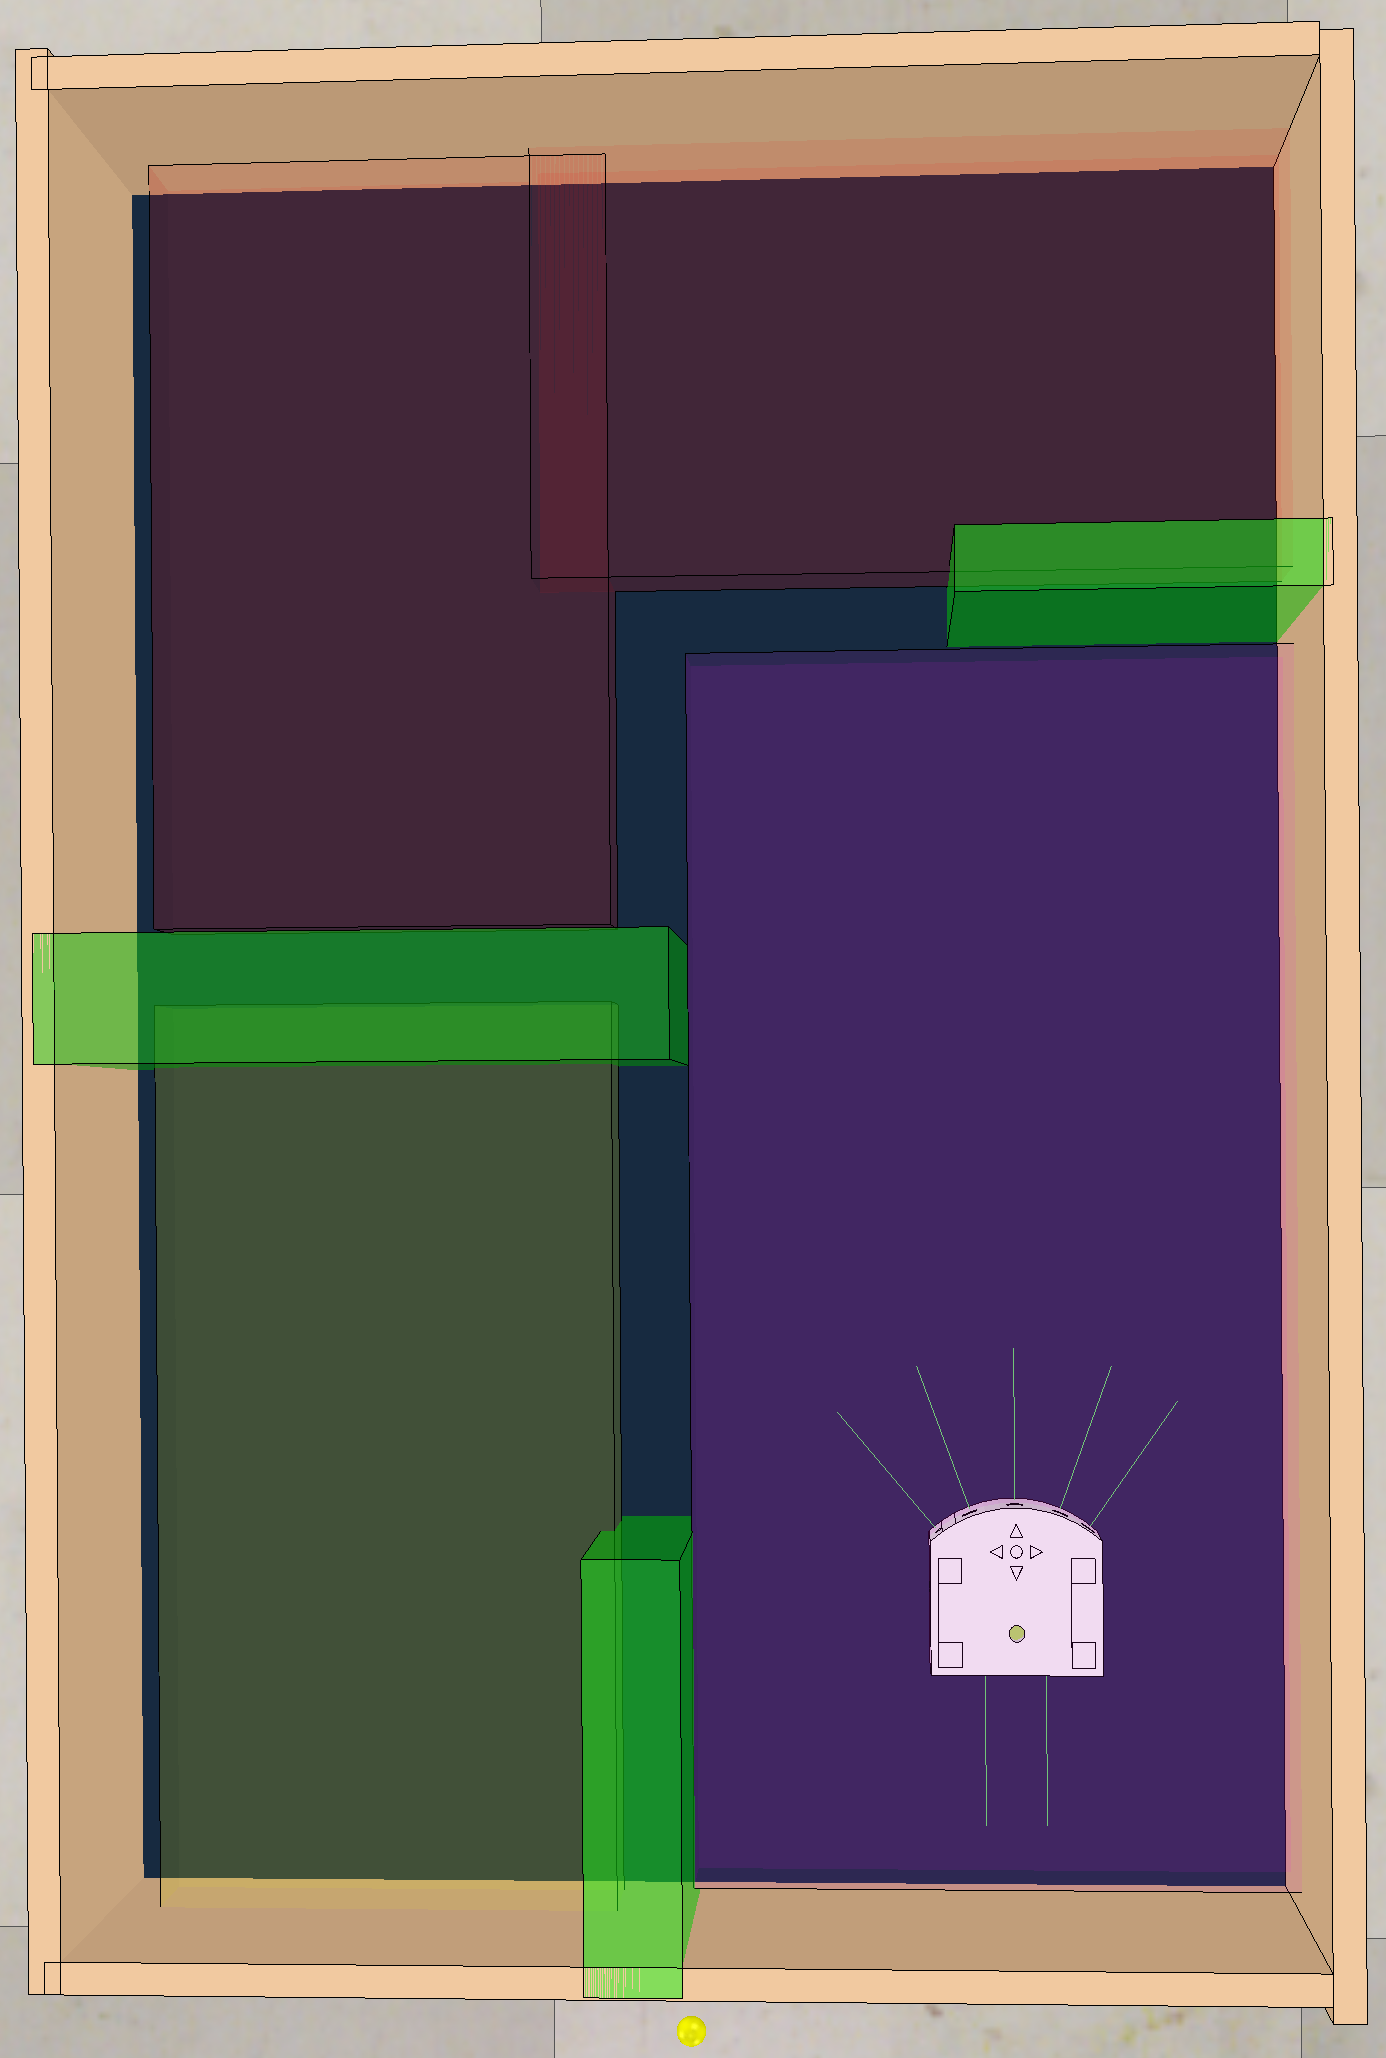
\includegraphics[width=1.0\linewidth]{include/images/virtual_arena.PNG}
  \caption{\label{fig:virtual_arena}Virtual Arena}
\end{minipage}
\end{figure}

\subsection{Obstacles}

Each arena (\emph{physical arena} and \emph{virtual arena}), contains 3 different cuboids in sizes. These are the only environmental objects that the robots interact with. Obstacles in the \emph{physical arena} are heavy enough, therefore they are not knocked over by \tmph{Thymio} robot during a collision. Additionally, each obstacle is marked with a fiducial marker, in order to set the position of its counterpart \emph{virtual obstacle} in the \emph{virtual arena}.

\begin{figure}[H]
\centering
\begin{minipage}{.5\textwidth}
  \centering
  \includegraphics[width=1.0\linewidth]{include/images/obstacle_physical.PNG}
  \caption{\label{fig:physical_arena}Physical obstacle.}
\end{minipage}%
\begin{minipage}{.5\textwidth}
  \centering
  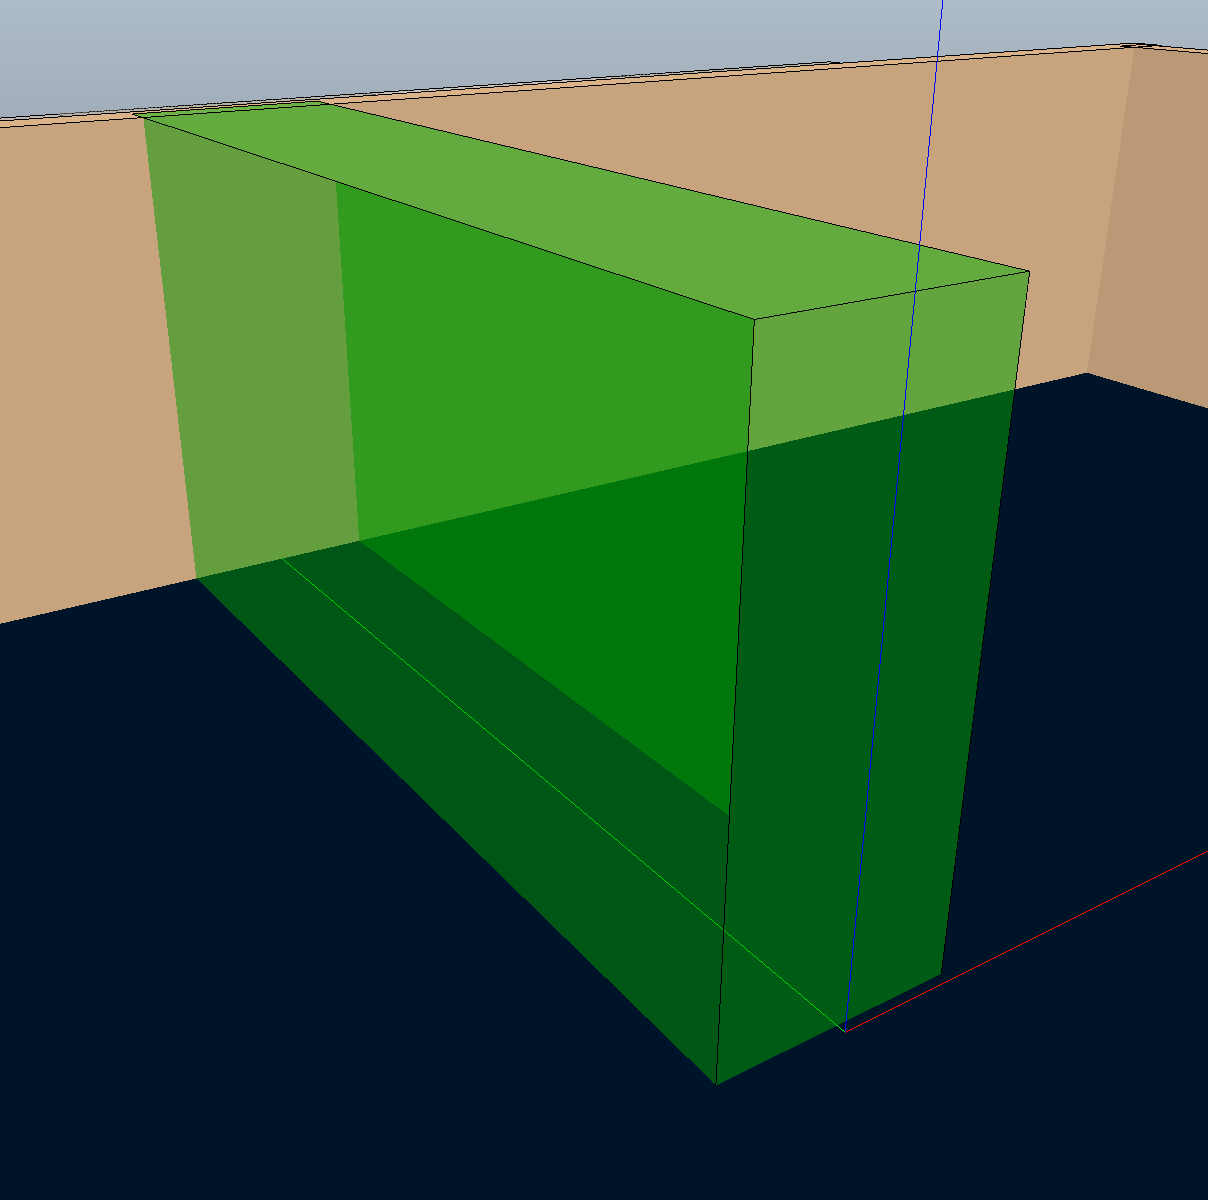
\includegraphics[width=1.0\linewidth]{include/images/obstacle_virtual.PNG}
  \caption{\label{fig:virtual_arena}The corresponding virtual obstacle.}
\end{minipage}
\end{figure}

\section{Robots}

One of the key component of our experiments is the physical robot. The main role that the robot system plays in our experimental setting is a black box to be programmed in order to create a concrete physical manifestation of the evolved robot control policies. In this case, the robot is not built, but rather a well functioning preassembled robot that serves as a supporting component. For our purposes, we focused on preexisting robotic platform, which comes with robot controller and programming environment, namely \emph{Thymio}.

\subsection{Thymio}

\emph{Thymio} \cite{mondada2017thymio} is a small robot produced by Mobsya\footnote{\url{http://www.mobsya.org/}} for educational purposes. It has 5 proximity sensors in front, 2 proximity sensors on the back as well as 2 grounds sensors. Thymio is also equipped with a temperature sensor, various buttons for interaction, visual sensors etc. A detailed overview of all the components can be seen in figure \ref{fig:thymio}. For this experiments purposes, we use the new \emph{Wireless Thymio}, which enables us to control the robot with a wireless dongle.

\begin{figure}[H]
\centering
\begin{minipage}{.5\textwidth}
  \centering
  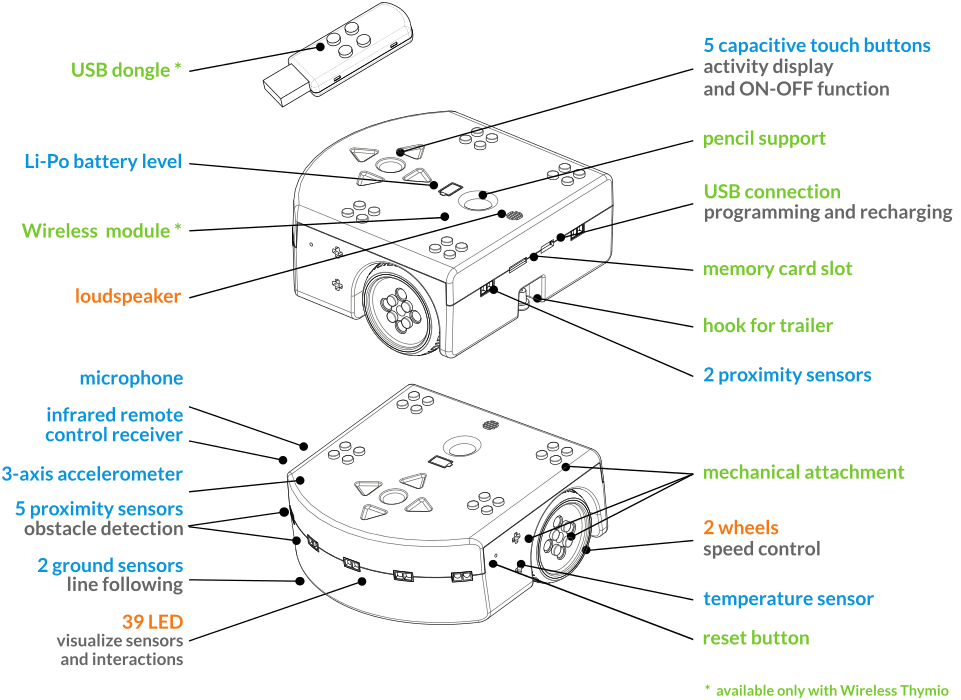
\includegraphics[width=1.0\linewidth]{include/images/thymio.PNG}
  \caption{\label{fig:thymio}Components of Thymio}
\end{minipage}%
\begin{minipage}{.5\textwidth}
  \centering
  \includegraphics[width=1.0\linewidth]{include/images/thymio_1.PNG}
  \caption{\label{fig:real_thymio}Thymio II model with attached powerbank}
\end{minipage}
\end{figure}

Thymio robot supports autonomous charging, between 4 and 5 hours of autonomy. In order to evaluate a single evaluation run without any intervetion, we placed a powerbank on top of the thymio. The main characteristics of the Thymio robot is summed up in this table:

\begin{table}[ht]
\centering
\begin{tabular}{|c|L{0.8\textwidth}|}
\hline
Characteristics & \multicolumn{1}{c|}{Values} \\ \hline
\texttt{Length} & 112 mm \\
\texttt{Width} & 117 mm \\
\texttt{Height} & 53 mm \\
\texttt{Weight} & 250 g \\
\texttt{Max. speed} & 0.2 m/s \\
\texttt{IR Sensors} & front.prox.horizontal.[0-4], back.prox.horizontal.[5-6], prox.ground.[0-1]; Proximity sensor response values between range 0-4500;  \\
\texttt{Battery} & Li-Po Battery: 3.7 V, 1'500 mAh, chargeable through microUSB port; Autonomy between 4 and 5 hours \\ \texttt{Powerbank} & 5'500 mAh, chargeable through microUSB port; Autonomy around 23 hours \\ \hline

\end{tabular}
\caption{The main characteristics of the Thymio II model}
\label{tabla_parametros}
\end{table}
\FloatBarrier

\section{Software Architecture}

\subsection{Aseba}

Thymio can be programmed with \emph{Aseba} \cite{retornaz2013seamless}, which is a set of tools that enables to program the robot within several programming environments, namely \emph{Visual, Blockly, Text, Scratch} programming. Aseba is shipped with a command-line utility tool called \emph{asebamedulla}, that allows accessing an Aseba network through \emph{D-BUS}\footnote{\url{https://www.freedesktop.org/wiki/Software/dbus/}}. This enables to program Aseba-enabled devices, the Thymio robot, using third-party languages. Since our preferred language is Python, the python CLI\footnote{\url{https://github.com/aseba-community/aseba/blob/master/examples/clients/python-dbus/aseba.py}} was chosen, which is a thin wrapper around asebamedulla dbus interface.

D-Bus is the main IPC system used in Linux: processes expose objects with a declared interface whose methods can be called from other processes. This is implemented by sending messages over D-Bus itself. The Aseba environment provides a D-Bus interface via the asebamedulla utility, which is in charge of transmitting to the robot hardware. The abstraction is in the form of a network of Thymio robots and processes listening on D-Bus, the so-called \emph{AsebaNetwork}.

The goal of the Aseba D-Bus integration is not to be an alternative to any of the Aseba languages used to program the robots locally. Indeed, it is meant to provide integration with another system, on which not only the D-Bus deamon and asebamedulla are running, but also the programs utilizing the D-Bus interface, which are never transferred in any manner to the Thymio hardware. This, in turn, means that the thymio is continuously connected to the machine on which the Python script, in our case, is running.

The API consists ultimately in the interfaces that asebamedulla provides over D-Bus. Through this interface, we can retrieve information about the network, read and write variables, or send events.

\begin{lstlisting}[style=C-color, caption={The API that asebamedulla provides over D-Bus},label={Asebamedulla API}]

interface ch.epfl.mobots.EventFilter {
    method Void ListenEvent(UInt16 eventId)
    method Void ListenEventName(String eventName)
    method Void IgnoreEvent(UInt16 eventId)
    method Void IgnoreEventName(String eventName)
    signal Event(UInt16 id, String name, Array<SInt16> payloadData)
}

interface ch.epfl.mobots.AsebaNetwork {
    method Void LoadScripts(String fileName)
    method Array<String> GetNodesList()
    method Array<String> GetVariablesList(String nodeName)
    method Void SetVariable(String nodeName, String variableName, Array<SInt16> variableData)
    method Array<SInt16> GetVariable(String nodeName, String variableName)
    method Void SendEvent(UInt16 eventId, Array<SInt16> payloadData)
    method Void SendEventName(String eventName, Array<SInt16> payloadData)
    method ObjectPath CreateEventFilter()
}
\end{lstlisting}

The \emph{AsebaNetwork} interface allows working with all of the nodes (robots) in the same network. There are methods to retrieve a list of the connected nodes ( \emph{GetNodesList} ) and to broadcast a global event, like \emph{SendEvent}. Global events are events that aseba nodes exchange within the aseba network. On the other hand, events that are internal to the node are called \emph{local events}. \emph{SetVariable} and \emph{GetVariable}, which write and read respectively native variables of the Aseba scripting language.

Asebamedulla exposes the interface \emph{EventFilter} which allows managing events. An application that wants to listen to events have register events with \emph{ListenEventName} or \emph{ListenEvent} be notified when an event occurs. The application can receive these events through the \emph{Event} signal, these events correspond to the global events of the Aseba language.

\subsection{Robotic Simulator}

In our experiments, a set of tools is needed in order to develop, test and validate different approaches to the reality gap problem. In relation to evolutionary robotics, these tools represent robotic simulators and robotic frameworks. Robotic simulators help to build the bridge between simulation and reality, they endorse that the developed simulation can be transferred and applied to real robotics. The most well know simulators in the community are \emph{V-REP} \cite{rohmer2013v} and \emph{Gazebo} \cite{koenig2004design} based on a survey made by Ivaldi, Peters, \cite{ivaldi2014tools}. These two simulators are compared in basic robotic control logic and evolutionary robotics experiment in \cite{nogueira2014comparative}. \emph{V-REP} robot simulation framework came out as the more intuitive and user-friendly simulator, which comes with various features and is less hardware demanding. Moreover, we have experience with \emph{V-REP} from previous works, therefore it was chosen as our main robotic framework.

In this work the use of V-REP simulation is not only used for \emph{Simulation-based optimization} and \emph{Robot-in-the-loop simulation-based optimization} approaches but also for \emph{Reality-based optimization} approach. V-REP exposes a remote API that allows controlling the simulation from the external client-side application. The client-side application is written in python which enables to control the simulation over the simulation variables.

\subsection{Computer Vision}

One of the most pivotal points of the computer vision is to track the Thymio robot during evaluation and positioning of the obstacles in the simulation. Therefore it goes without saying that the system must be able to accurately read the position and angle of these objects. Since the environment is static and small in size, a fixed-camera computer vision is optimal to extract the necessary spatial information within a single image. The most necessary problem is solving the objects identification and accurate spatial information extraction. These problems are usually dealt with using certain marker systems. One of such a system is \cite{bencina2005improved}, which relies on 2D tracking of specially designed fiducials (markers) in a real-time video stream. This system involves a set of marker patterns and computer vision algorithms that can track and yield various spatial information of these markers. Such a marker system was chosen in this project as it perfectly satisfy our requirements. The choice is supported by the same computer vision system being used and proven in \cite{faina2017automating}.

\subsubsection{Fiducial tracking}

The \epmh{ReacTIVision Fiducials} \ref{fig:fiducial_markers} comes in 3 different set of sizes \emph{small, medium, large} and each individual marker has it's own unique id. Furthermore, each of them is purely identified by its unique topological structure. The system employs the topological fiducial recognition, which enables detection and identification. In this approach, a region adjacency graph is computed from a binary image. The adjacency graph can be understood as a tree. By recognizing the graphs representing the fiducials, markers can be detected and identified. Moreover, the location is computed as the weighted average of all leaf centers (black and white). The vector from this centroid to a point given by the weighted average of all black (or white) leaf centers is used to compute the orientation of the fiducial \cite{bencina2005improved}.

\begin{figure}[H]
  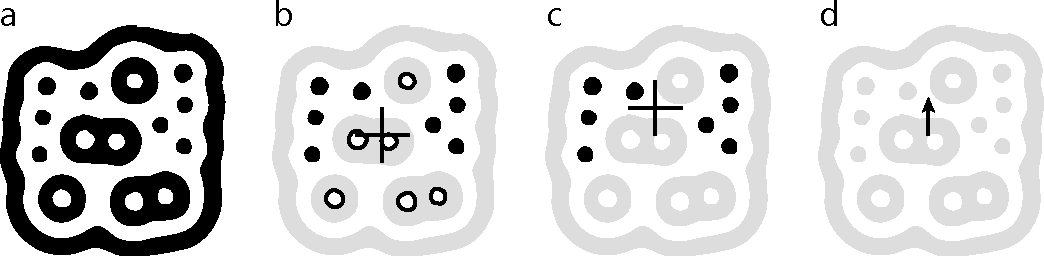
\includegraphics[width=0.66\linewidth]{include/images/fiducial_markers.PNG}
  \caption{\label{fig:fiducial_markers}ReacTIVision Fiducials from original paper a) a reacTIVision fiducial (b) black and white leafs and their average centroid (c) black leafs and their average centroid, and (d) the vector used to compute the orientation of the fiducial}
\end{figure}

\subsubsection{Computer Vision Implementation}

The original implementation of the \emph{reacTIVision} system has been re-implemented using \emph{OpenCV}\footnote{\url{https://opencv.org/}} by Faina, in \cite{faina2017automating}. The actual implementation is written in Python, and have been slightly modified, concretely, have been made thread-safe. The entire vision system operates on pixel-coordinates, which is turned into a base coordinate system. Transformation...

The video frame is captured by using an HD camera \footnote{Logitech 1980x1080 pixels}, which is placed on top of the physical arena \ref{fig:test_bed}. Processing a single frame consist of the following steps: 

\begin{itemize}
  \item Pre-processing. Compensate radial and tangential lens distortion.
  \item Thresholding. Transform grayscale image to a binary image.
  \item Segmentation. Construct the region adjacency graph.
  \item Fiducial Recognition. Subgraphs are identified and their location and orientation are computed.   
\end{itemize}

As was pointed out in \cite{faina2017automating}, the lighting condition has to be constant in order to be able to locate the fiducial markers. This issue arises only when sudden, lighting changes occur in the environment. For example, window blinds have been folded. Even though the vision system is able to compensate incidents such this by stabilizing the image, when the lighting conditions are too extreme (sunset/sunrise) the cameras automatic white balancing and focusing make the image to blurred to identify the fiducial markers. This issue was fixed by placing a fixture to the ceiling which ensured that the lighting condition is more or less constant.


\subsection{Simulation Restart}

One of the requirements of the evolutionary procedure applied in this projects is that the agent is required to start each iteration of the evolutionary algorithm from the same position. Naturally, for the simulation-based approach utilized in a simulation, it is not a problem, since the robot position can be easily set by the simulation tool. On the other hand, this behavior had to be implemented in the reality-based optimization approach for dealing with situations when the Thymio had to return to his initial position after an evaluation. This behavior is the \emph{path following} behavior of the Thymio vehicle. Several important facts had to be considered in the implementation. Among the most important one is the ability to track the path from any given position to the initial position. In addition to this tracking, the system has to take full control of the Thymio vehicle and operate it to follow the computed route as close as possible to the initial position, considering all errors along the way. Another important part of the path following is the consideration of the obstacles. It has to take into account the static obstacles that might be in the direction of travel.

\subsubsection{Path following}

\section{Automation Control}

\subsection{Evaluation of the robotic platform}

\chapter{Experiments}

All our reality gap approaches have been validated on a robotic application with the Thymio robot on an obstacle avoidance task. The experimental set up among all approaches mainly differ in the evolutionary strategy used or whether the optimization happened fully or partially in simulation and reality. The following next paragraphs describe the common set-up used in our experiments.

The robot is quipted with 7 infrared sensors and 2 two motors. The virtual thymio robot is modeled based on the physical thymio and its characteristics \ref{thymio_characteristics}. The specifications of sensor readings and possible speed values, included normalization values are depicted in the following table \ref{fig:thymio_specs} both for the physical thymio and its virtual counterpart.

\begin{table}[H]
\begin{tabular}{llll}
\centering
\hline
\textbf{}                            & \textbf{Simulator}    & \textbf{Reality}  & \textbf{Normalized}  \\ \hline
\textbf{Speed Values}                & {[}-2.0, 2.0{]}       & {[}-200, 200{]}      & {[}0.0, 1.0{]} \\
\textbf{Sensory Readings}            & {[}0.0, 1.0{]}        & {[}0, 4500{]}        & {[}0.0, 1.0{]} \\
\end{tabular}
\caption{The Thymio robot sensors and speed values specification.}
\label{tab:thymio_specs}
\end{table}

The evaluation of a single genome takes 60 simulation seconds for the simulation-based approaches and 60 wall clock seconds for the reality-based approaches from a fixed initial position each test. At each step (50ms), the Thymio robot sensory readings are fed to the neural network and the network outputs are multiplied by the maximal wheel speed and used to apply to the wheels of the Thymio robot. The network outputs are in the range of \emph{0.0} and \emph{1.0}, and since the Thymio can move backward, the output values are transformed into a positive/negative range where \emph{0.5} is the point of direction inversion. In order to speed up the optimization, the evaluation of a genome is stopped if the system detects that the robot collided with the walls or the environmental objects. Furthermore, if the robot is not moving or spinning in one place the evaluation is stopped and the fitness is calculated over reduced simulation time.

The fitness function relies on a set of features that can be measured within the interaction between the robot and its environment. Hence the fitness function relies on 3 features, as follows:

\begin{enumerate}
    \item \(V_{t} = \frac{V_{l} + V_{}r}{2} \) \textbf{Average wheel speed} of both wheels at a particular timestamp \emph{t}.
	\item \((1-\sqrt{\Delta v})\) \textbf{The algebraic difference} between the speed values at a particular timestamp \emph{t}. The smaller is the difference, the faster the robot moves.
	\item \((1 - P_{t})\) \textbf{Max Sensor activation} the activation value of the proximity sensor with the highest activity. The closer the robot is to the walls or obstacles the less fitness it accumulates.
\end{enumerate}

The fitness function \ref{eq:fitness_function} is defined as a dot product of all these features divided by the fixed simulation time. 

\begin{equation}
	f = \sum_{t=1}^{t_{max}} \frac{V_{t} (1 - \sqrt{\Delta v}) (1 - P_{t})}{60}
	\caption{Task dependent fitness function}
	\label{eq:fitness_function}
\end{equation}

For each evaluated controller, we extract certain \emph{behavioral feautures} \ref{eq:behavioral_features} during the optimization process. These features allow us to describe/quantify the behavior of each controller. Moreover, it allows us to compare controllers in a simple manner without any dependency on the evolutionary strategy applied or the controller's genotype. The 12-dimensional features are defined as 1) the average left and right wheel speeds 2) the average value of each sensor activation 3) percentage of time spent in each section of the arena throughout the evaluation. These features are normalized in the range of \emph{0.0} and \emph{1.0}.

\begin{equation}
	b_{controller} = [avg_{left}, avg_{right}, s_{1}, s_{2}, s_{3}, s_{4}, s_{5}, s_{6}, s_{7}, area_{0}, area_{1}, area_{2}]
	\caption{12-dimensional behavarioral features}
	\label{eq:behavioral_features}
\end{equation}

Additionally, we extract the position of the Thymio robot during evaluation. The vision system is used to extract the position from reality and the system is responsible for the position from the simulation. This feature measure is used to qualify a given controllers transfer from simulation to reality.

\section{Simulation-based optimization}

Our first application aims to explore the \emph{simulation-based optimization} approach to the reality gap problem. The first part of the experiments involves evolving an obstacle avoidance behavior in simulation. Finding the right parameters of the evolutionary strategy to achieve optimal obstacle avoidance behavior, like, number of generations, population number, etc. The second part is focused on the transferability of controllers. Taking the best controllers evolved in simulation and validate how well they transfer to reality. Additionally, this approach is later compared to the reality-based optimization approach to the same application.

\subsection{Experimenal design}

The first experiment takes place fully in simulation using the simulation model mentioned earlier \ref{fig:virtual_arena}. The aforementioned evolutionary algorithm applied in this experiment is \emph{NEAT} \citep{stanley2002evolving}. A controller, in this case, the genome, is represented as a neural network. The implementation is based on the python-neat \footnote{\url{https://neat-python.readthedocs.io/en/latest/}} library which has been modified to fit our requirements. The genome contains a list of \emph{connection genes} and list of \emph{node genes}. Node genes encode the input, hidden nodes, and outputs of the neural network that can be connected. Whether a node is connected to other node is expressed in the connection gene. The initial neural network structure consists of 7 input nodes (each represents the infrared sensors placed around the Thymio), fully connected to the 2 motor neurons computing the speeds of the wheels. This way the algorithm starts with a fixed topology and by applying the biological operators over generations it may evolve. In the early stage of the experiments various parameters of the evolution have been tested (population size, generations, mutation rate, etc.), but the most promising results have been achieved by the parameters summarized in table \ref{tab:neat_parameters}. The experiment have been reproduced 10 times.

\begin{table}[H]
\centering
\begin{tabular}{ll}
\hline
\textbf{}                      & \textbf{} \\ \hline
\textbf{Population size}       & 20        \\
\textbf{Number of generations} & 20        \\
\textbf{Simulation time}       & 60 sec    \\
\textbf{Activation function}             & sigmoid       \\
\textbf{Connection add probability}              & 0.5       \\
\textbf{Connection delete probability}              & 0.5       \\
\textbf{Node add probability}              & 0.2       \\
\textbf{Node delete probability}              & 0.2       \\
\textbf{Elitism}  & 1      
\end{tabular}
\caption{Parameters of the NEAT algorithm.}
\label{tab:neat_parameters}
\end{table}


\subsection{Results}

Figure \ref{fig:sim_avg_fitness} shows the average fitness performance of 10 simulation runs in simulation. The optimality of any given controller is hard to determine since the fitness is simply maximized. However, it is clear from the figure that the fitness is progressing towards some optimum. Furthermore, figure \ref{fig:sim_best_genomes_percentile} shows the performance of the best genomes in each generation across all simulation runs. In addition, it shows the median and 25\%/75\% percentiles. The smooth max curve in some generations is the evidence of elitism in the NEAT algorithm set up. 

\begin{figure}[H]
    \centering
    \begin{subfigure}[b]{0.8\textwidth}
    	\centering
        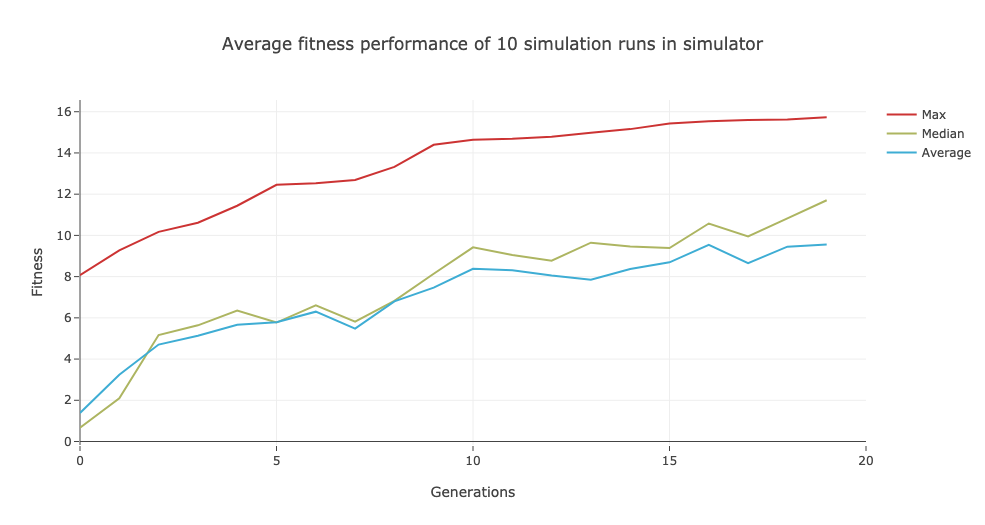
\includegraphics[width=5cm]{include/images/sim_avg_fitness.PNG}
        \caption{Average fitness of 10 simulation runs}
        \label{fig:sim_avg_fitness}
    \end{subfigure}
    \begin{subfigure}[b]{0.8\textwidth}
    	\centering
        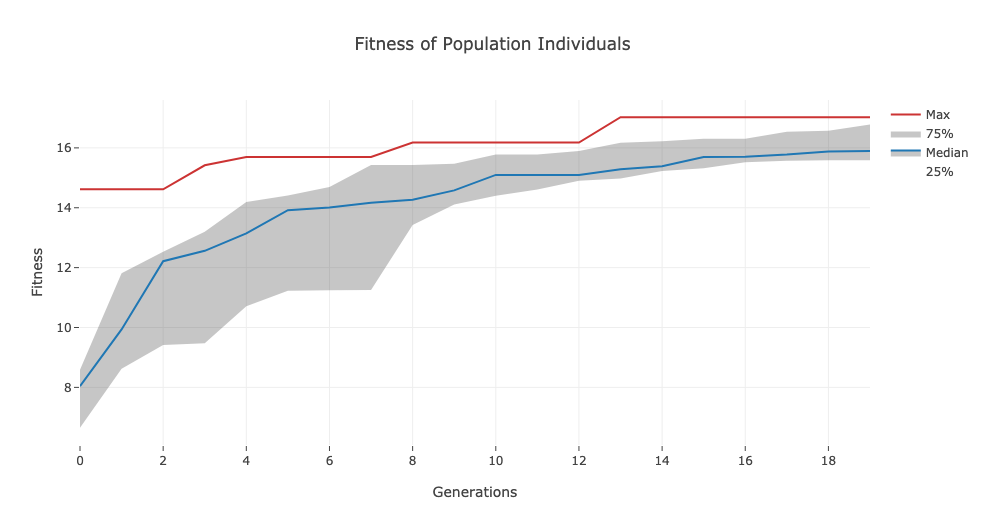
\includegraphics[width=5cm]{include/images/sim_best_genomes_percentile.PNG}
        \caption{Best controllers each generation over all the runs.}
        \label{fig:sim_best_genomes_percentile}
    \end{subfigure}
    \caption{Simulation based results I.}
	\label{fig:sim_based_resultsI}
\end{figure}

Figure \ref{fig:sim_fitness_distribution} shows the distribution of each individual in the population for a single simulation run. Each evolutionary run took on average \~4 hours, thus \~40 hours in total. The objective was to evolve controllers that exhibit obstacle avoidance behavior. The visual manifestation of behaviors is depicted in figure \ref{fig:sim_path_travelled}. It shows the path taken by the best genomes in each simulation run. It is noticeable that each controller moves forward until it makes a sharp turn to the left to avoid a collision with an obstacle. To further validate the robustness of best controllers, the obstacles in the simulation where randomly misplaced from their initial positions, and each genome was post-evaluated in a slightly new environmental set-up. Again all the genomes exhibited the desired obstacle avoidance behavior. This showcase that the evolved controllers are able to generalize.

\begin{figure}[H]
    \centering
    \begin{subfigure}[b]{0.8\textwidth}
    	\centering
        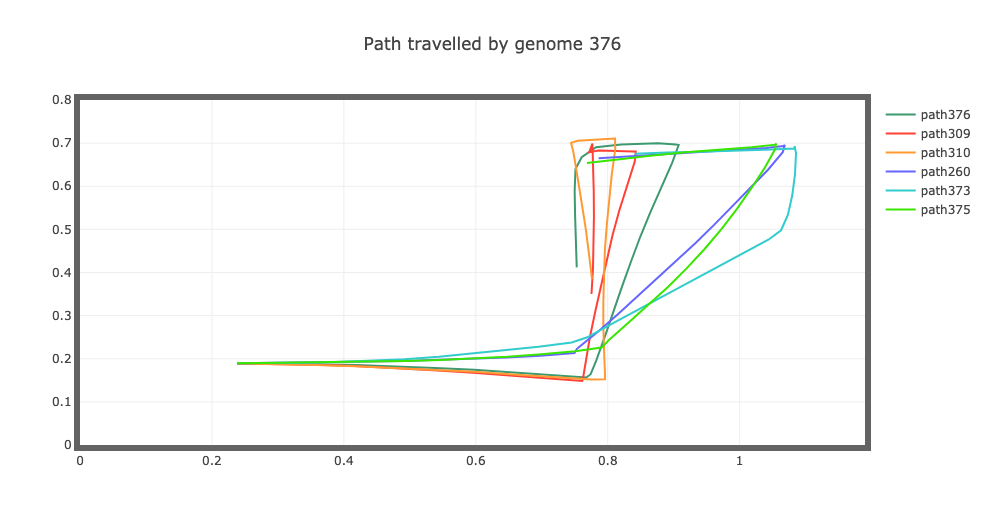
\includegraphics[width=8cm]{include/images/sim_path_travelled.PNG}
        \caption{Path travelled by the best genomes.}
        \label{fig:sim_path_travelled}
    \end{subfigure}
    \begin{subfigure}[b]{0.8\textwidth}
    	\centering
        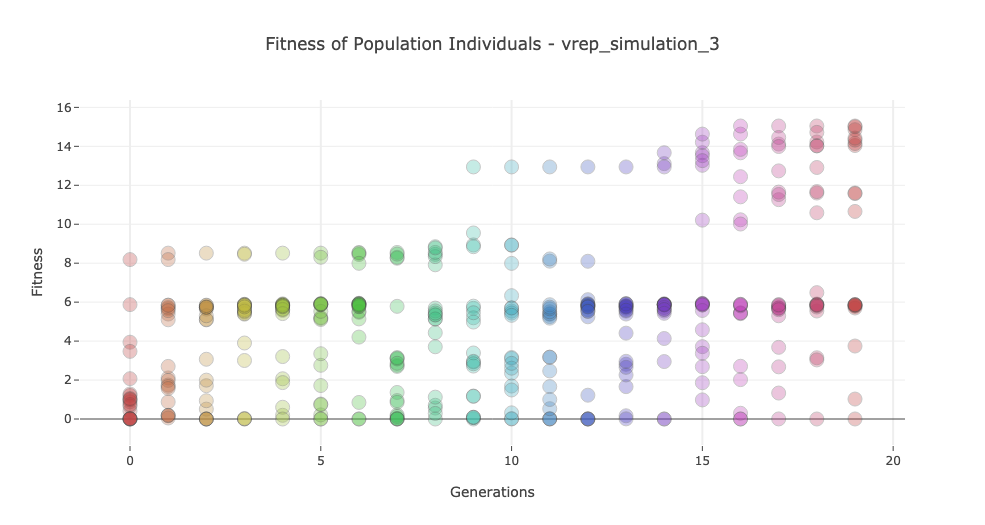
\includegraphics[width=8cm]{include/images/sim_fitness_distribution.PNG}
        \caption{Fitness distribution of population individuals for a single run.}
        \label{fig:sim_fitness_distribution}
    \end{subfigure}
    \caption{Simulation based results II.}
	\label{fig:sim_based_resultsII}
\end{figure}

Another interesting result concerns the behavioral features of the best genomes. As can be seen in figure \ref{fig:sim_behavioral_features_best}, it appears that all the genomes have almost the same behavioral values. The average wheel speed values indicates that the robots right wheel is set at full speed at evaluation while the right motor is not. This explains while the robot takes always left turns. Since the left motor is set to lower values than the right motor. Additionally, the front horizontal sensors (s1-s5) are the most active, while the back sensors (s6 and s7) are least active.

\begin{figure}[H]
    \centering
    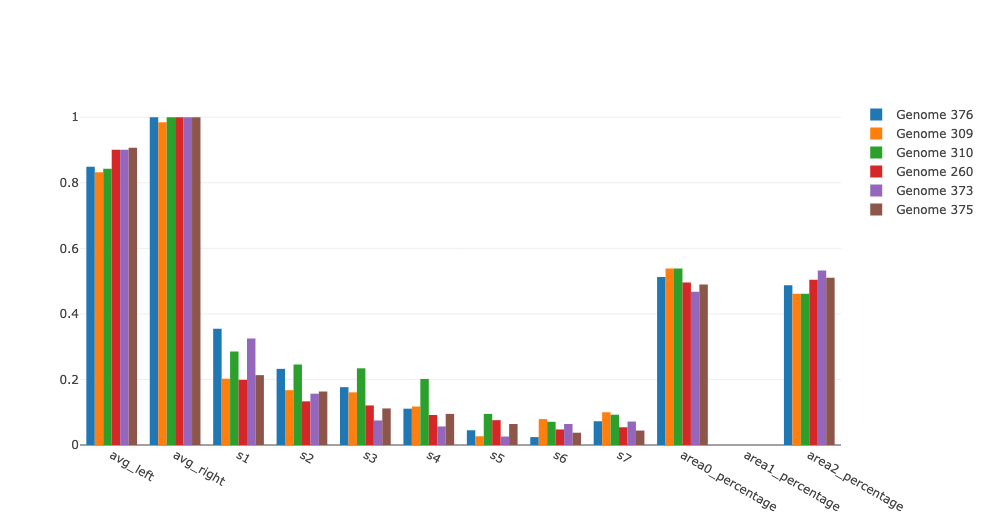
\includegraphics[width=8cm]{include/images/sim_behavioral_features_best.PNG}
    \caption{Behavioral features of the best genomes.}
    \label{fig:sim_behavioral_features_best}
\end{figure}

\begin{table}[h]
\centering
\begin{tabular}{ccc}
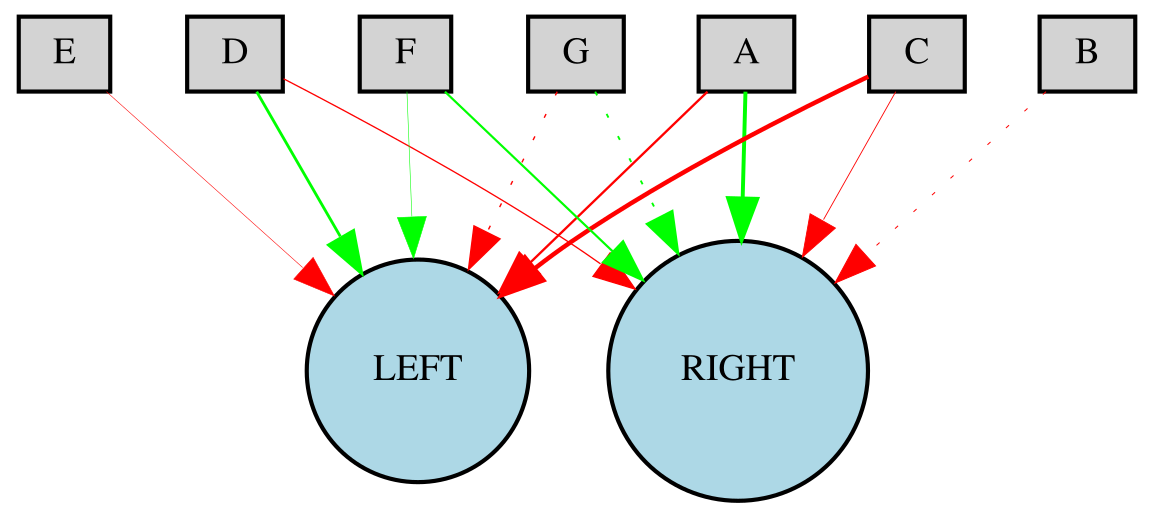
\includegraphics[scale=0.4]{include/images/sim_network_1.PNG} & 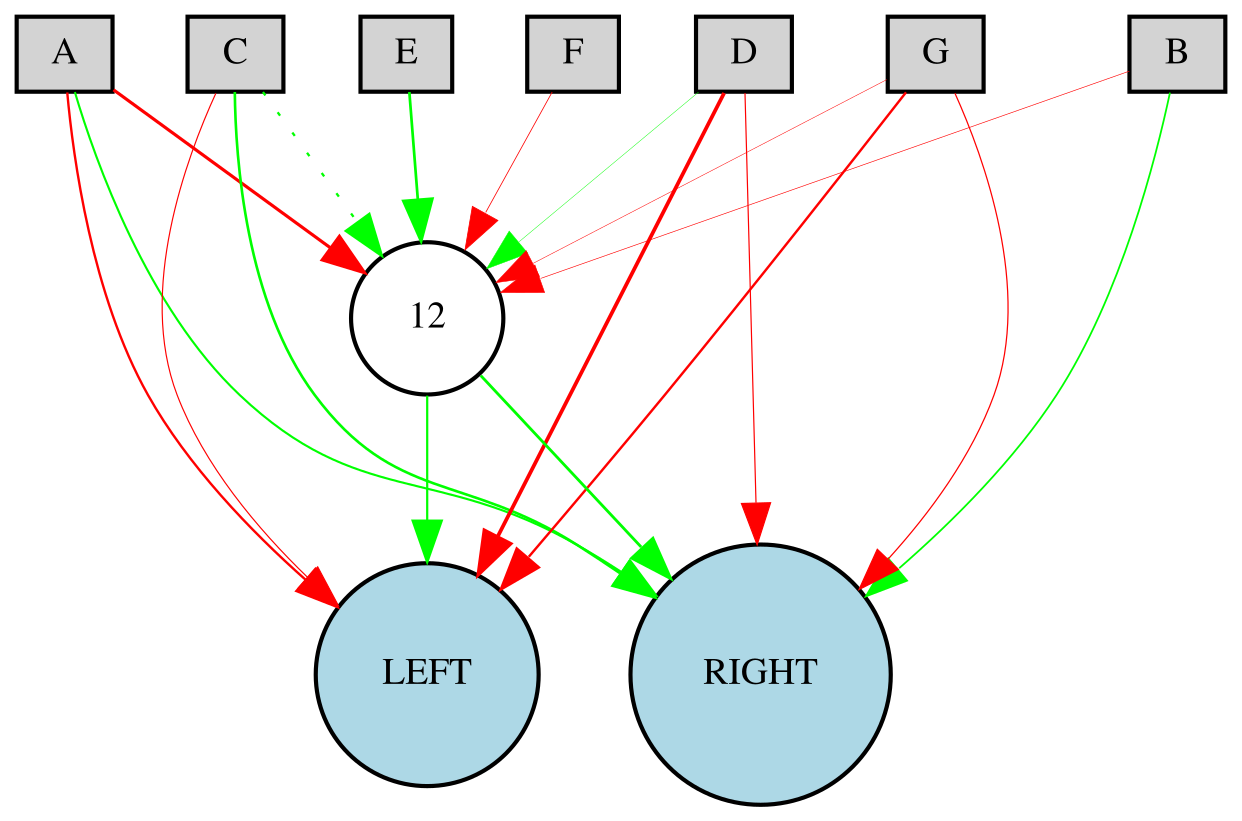
\includegraphics[scale=0.4]{include/images/sim_network_2.PNG} & 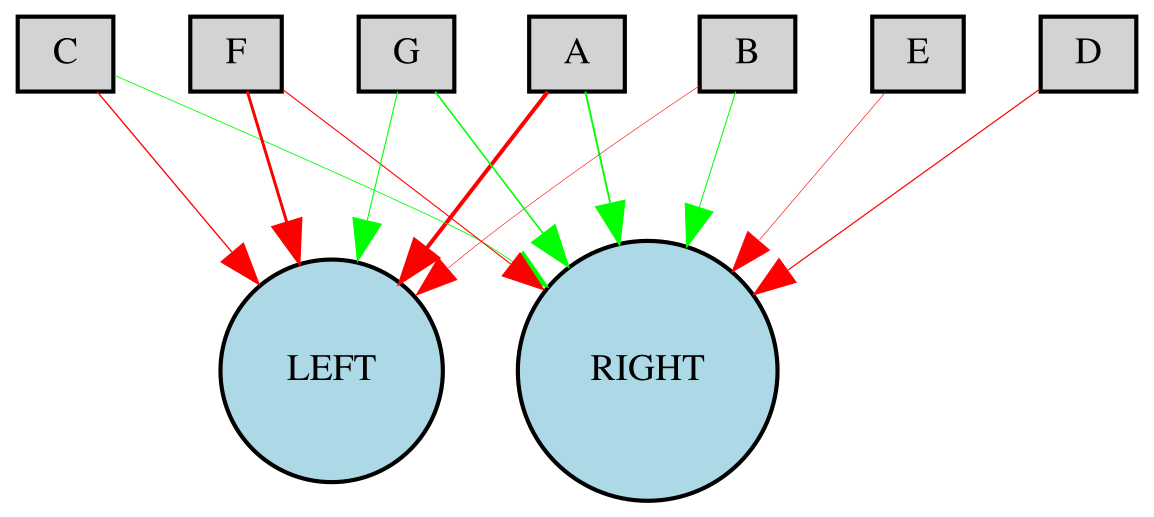
\includegraphics[scale=0.4]{include/images/sim_network_3.PNG} \\
$$Genome \;  \; 376$$  & $$Genome \;  \; 309$$  & $Genome \;  \; 310$  \\
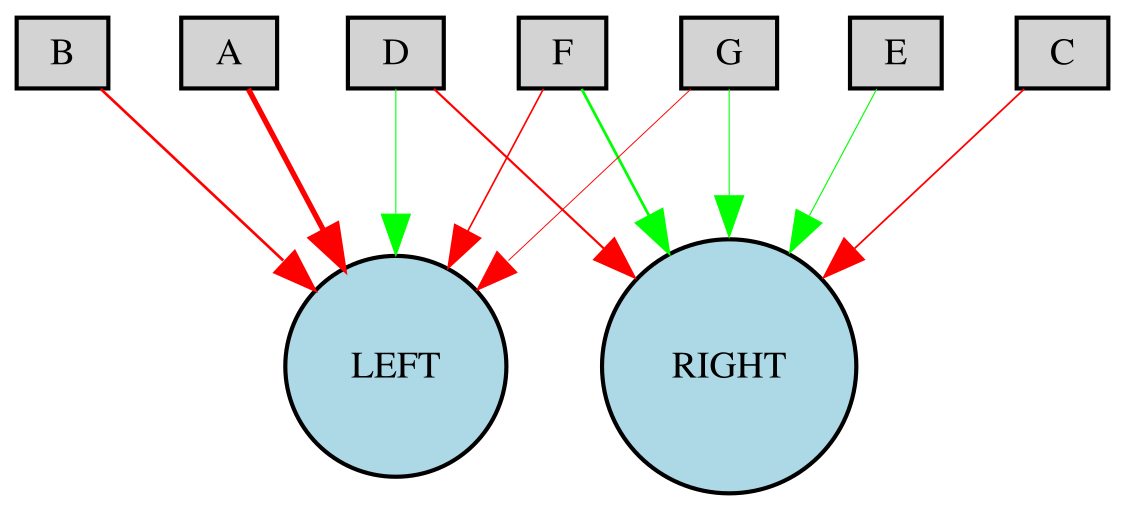
\includegraphics[scale=0.4]{include/images/sim_network_4.PNG} & 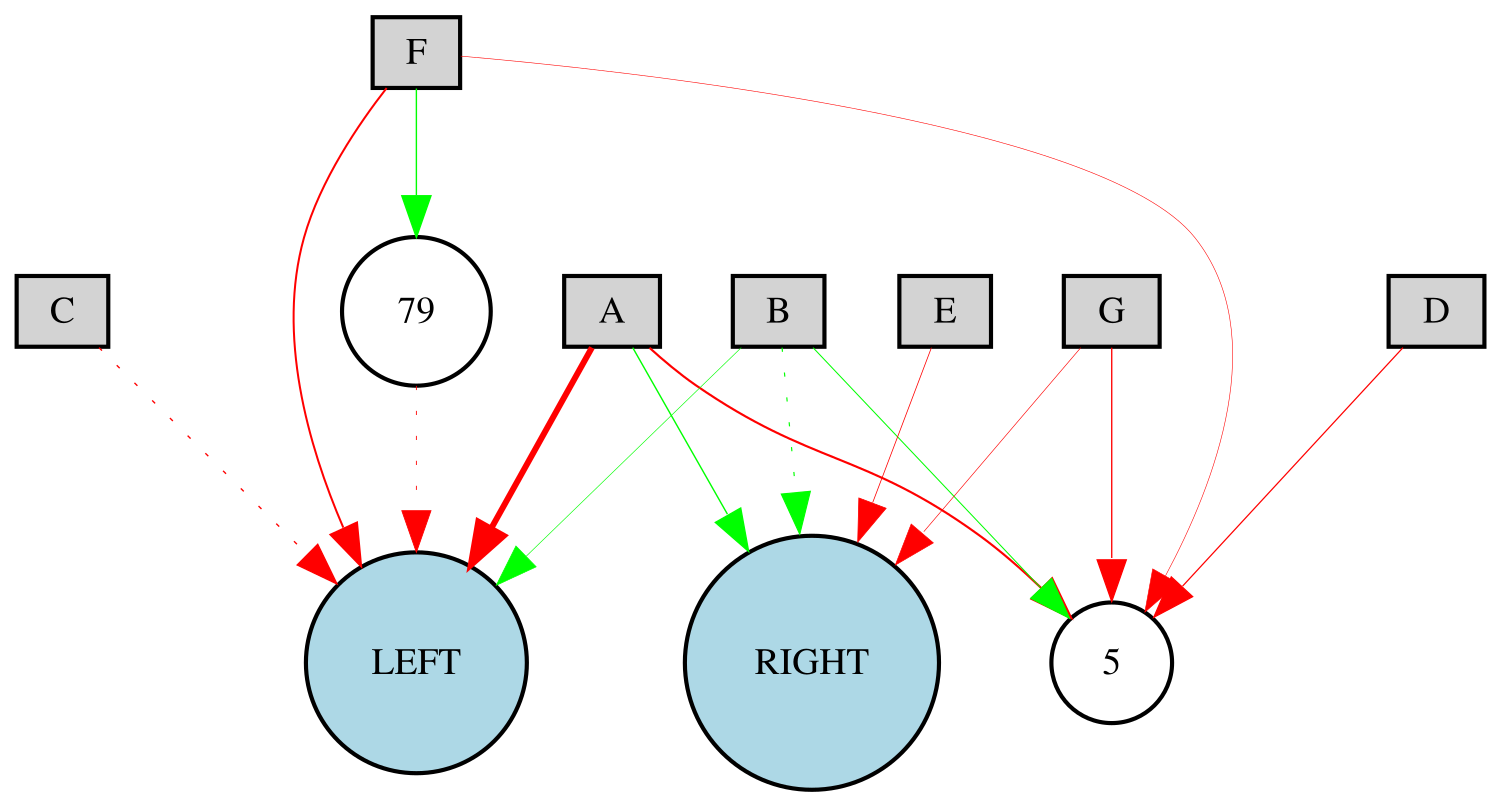
\includegraphics[scale=0.4]{include/images/sim_network_5.PNG} & 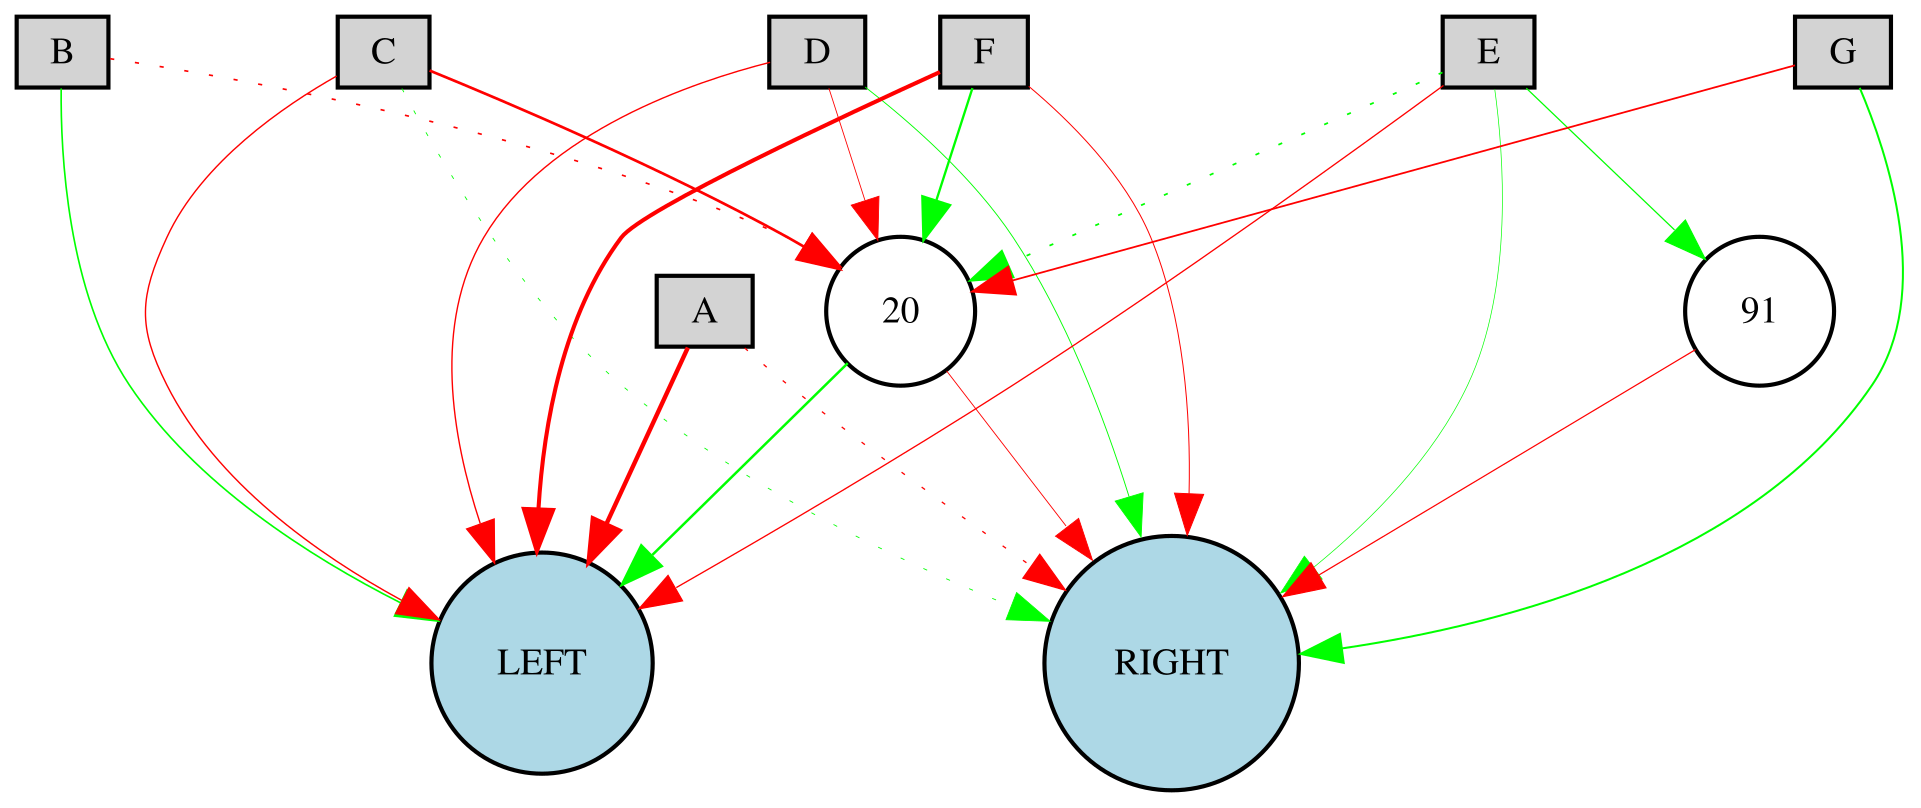
\includegraphics[scale=0.4]{include/images/sim_network_6.PNG} \\
$Genome \;  \; 260$  & $Genome \;  \; 373$  & $Genome \;  \; 375$  \\
\end{tabular}
\caption{Evolved topology of the best controllers in simulation.}
\label{fig:sim_network_topologies} % 
\end{table}

The evolved topologies of the neural networks can be seen in figure \ref{fig:sim_network_topologies}. The green and red color connections represent positive/negative weight values. Notice that not all the connections are enabled. The doted connections refer to connections that were disabled over time. In addition, the evolutionary process has evolved a hidden layer with 1 or 2 neurons in some cases (Genome 375, Genome 373 or Genome 309).

\emph{Transferability.} To validate and examine whether the evolved controllers in a simulation are transferable we took the best controllers from each simulation run and transferred them directly to the Thymio robot. For example, a behavior of the best controller transferred to reality is depicted in figure \ref{fig:sim_bad_transfer}. The trajectory of the controller in the simulator is shown with a dark green color. The transferred controller is post evaluated 10 times and its typical behavior consists of going straight without taking into account the obstacle in front. Among one of them (red) attempts to avoid the obstacle, however unsuccessfully as it afterward turns to directly to the obstacle and keeps colliding with it. It undoubtedly highlights that there is a reality-gap problem between simulation and reality. However, as it turned out this gap can be convoluted. Among the transfered controllers (10), we have identified 2 controllers that are transferable and able to avoid obstacles. A typical behavior of a transferable controller is picture on \ref{fig:sim_good_transfer}. This lead to a conclusion that there is a clear gap between simulation and reality, however, sometimes good solutions can be evolved in simulators that are transferable to reality.

\begin{figure}[H]
    \centering
    \begin{subfigure}[b]{0.8\textwidth}
    	\centering
        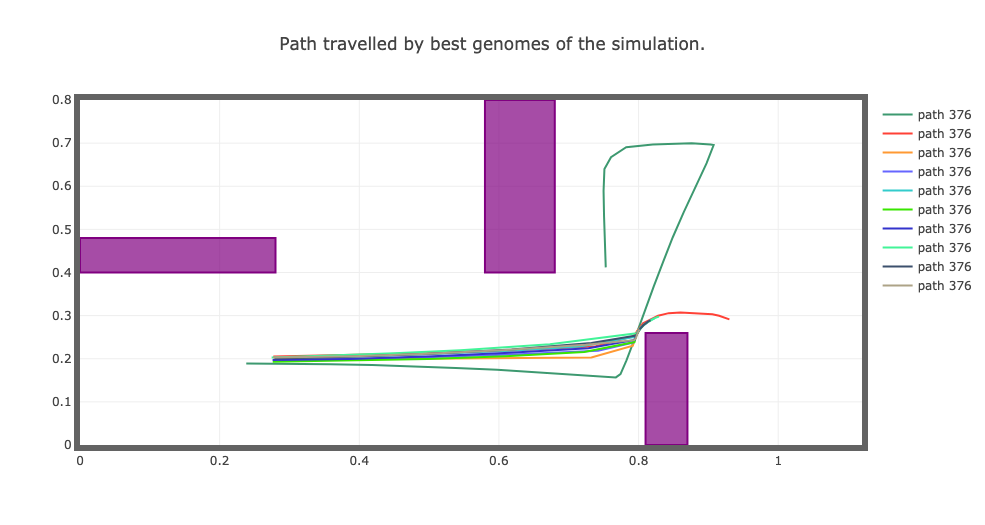
\includegraphics[width=8cm]{include/images/sim_bad_transfer.PNG}
        \caption{Controller that is not transferable.}
        \label{fig:sim_bad_transfer}
    \end{subfigure}
    \begin{subfigure}[b]{0.8\textwidth}
    	\centering
        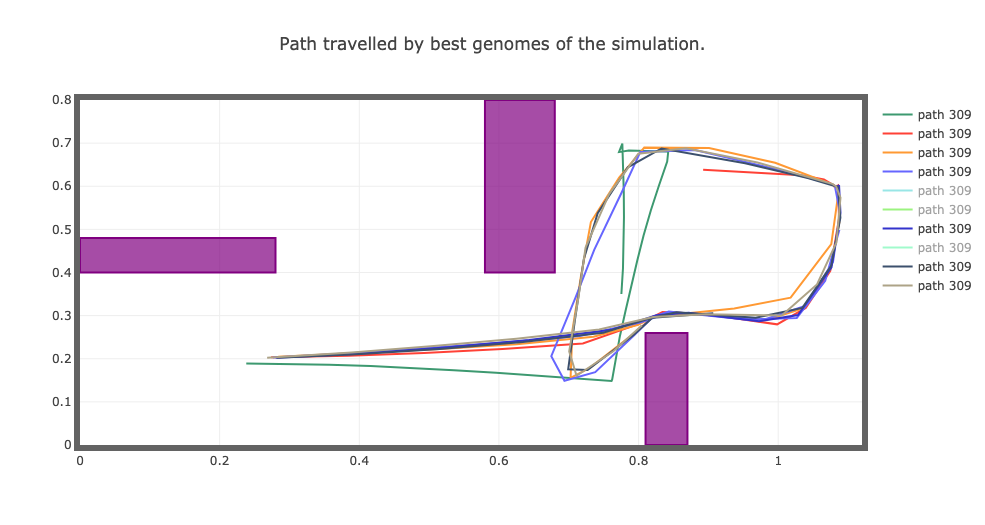
\includegraphics[width=8cm]{include/images/sim_good_transfer.PNG}
        \caption{Controller that transfered well to reality.}
        \label{fig:sim_good_transfer}
    \end{subfigure}
    \caption{Typical behaviors of the best controllers transferred to reality. Each of them post-evaluated 10 times in reality.}
	\label{fig:transferred_controllers}
\end{figure}

\section{Reality-based optimization}

\subsection{Experimenal design}

For comparison to the simulation-based optimization, we conduct a reality-based optimization directly on the physical robot. The experimental set-up is the same as in the previous application. The size of the population is 20 and the number of generations is 20. Again, NEAT is used as the underlying evolutionary strategy with the same parameters summarized in table \ref{neat_parameters}. It has been reproduced 10 times, which implies 4000 evaluations, to have the same amount of experiments in reality as in simulation. The experiment completely relies on the entire robotic platform including the vision system, simulation, and the Thymio robot.

\subsection{Results}

The summary of results are depicted in figure \ref{fig:real_based_resultsI}. The thymio evolved an obstacle avoidance behavior in less than 20 generations. Each simulation run taking  approximately 16 hours, thus 160 hours in total. Most of the best thymio controllers maintain a straight trajectory and perform right turns when necessaary. Like in the previous experiment, there is no clear way to differentiate between optimal solutions and non-optimal ones, the fitness is simply maximized. Looking at the figure \ref{fig:real_best_genomes_percentile} of the best controllers, it indicates that controllers with high fitness emerge by the 10th generation, even though the progress is not smooth as in the simulation-based optmization. However, the dips in the curves are the result of noise. Figure \ref{fig:thymio_network_topologies} shows the evolved topologies of the best 6 controllers.

\begin{figure}[H]
    \centering
    \begin{subfigure}[b]{0.8\textwidth}
    	\centering
        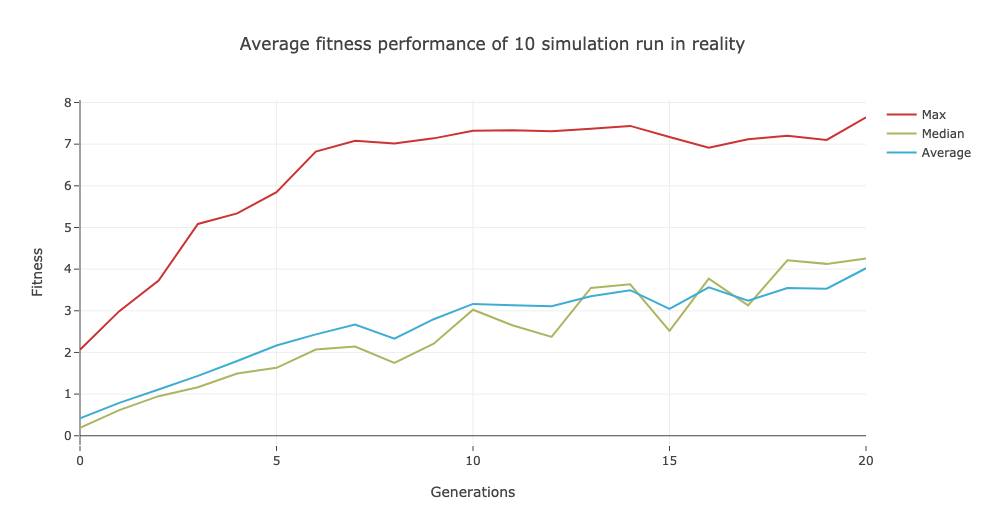
\includegraphics[width=5cm]{include/images/real_avg_fitness.PNG}
        \caption{Average fitness of 10 simulation runs.}
        \label{fig:real_avg_fitness}
    \end{subfigure}
    \begin{subfigure}[b]{0.8\textwidth}
    	\centering
        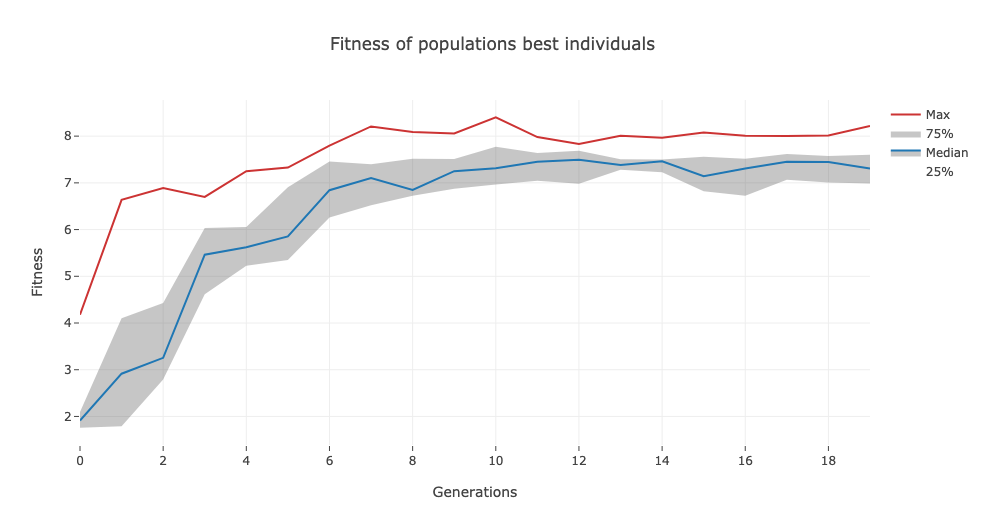
\includegraphics[width=5cm]{include/images/real_best_genomes_percentile.PNG}
        \caption{Best controllers each generation over all the runs.}
        \label{fig:real_best_genomes_percentile}
    \end{subfigure}
    \caption{Reality-based simulation results I.}
	\label{fig:real_based_resultsI}
\end{figure}

The corresponding behavior of 5 best controllers is depicted in figure \ref{fig:path_traveled_thymio_reality_based}. 2 of them have similar behavior, going straight and making a sharp \emph{U} turn after they sense the obstacle in front of them. On the other hand \emph{Genomes 189, 73, 24}, are taking a left turn and keep moving around in the the second area most of the time.


\begin{table}[h]
\centering
\begin{tabular}{ccc}
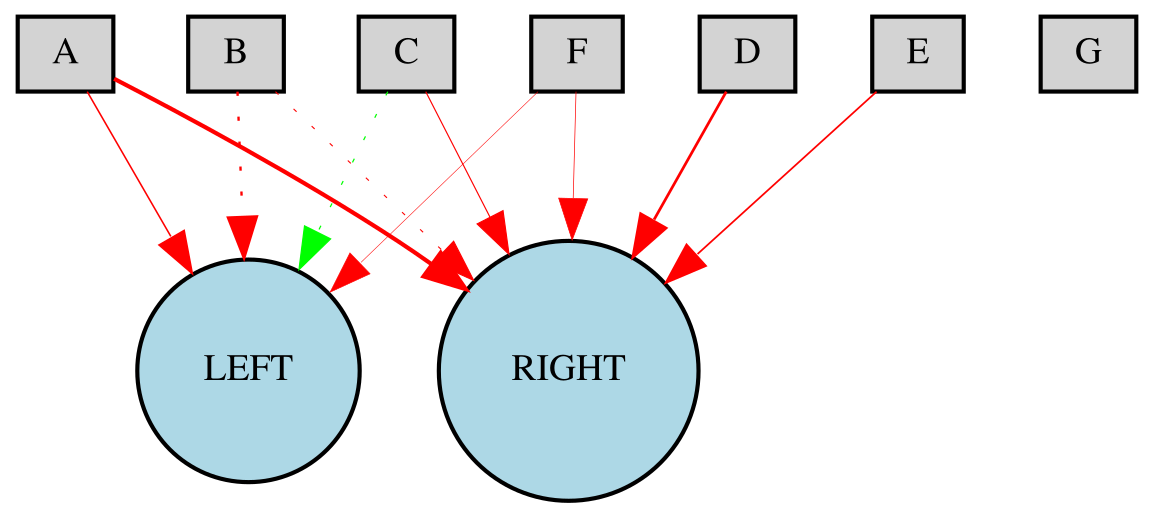
\includegraphics[scale=0.4]{include/images/thymio_network_379.PNG} & 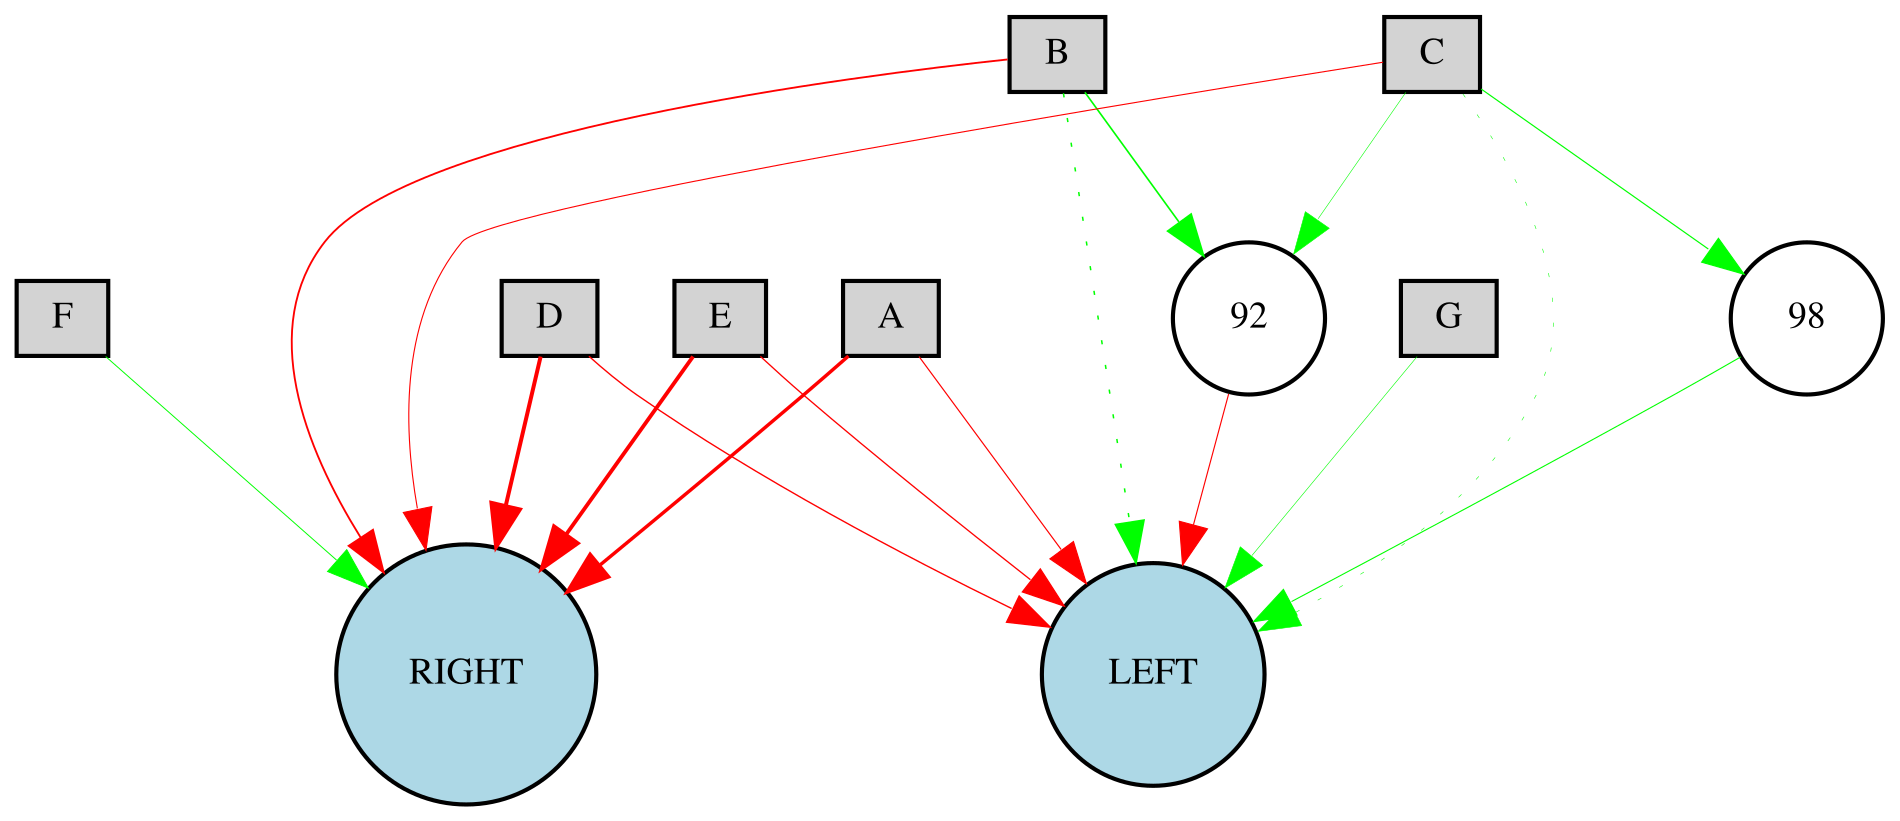
\includegraphics[scale=0.4]{include/images/thymio_network_78.PNG} & 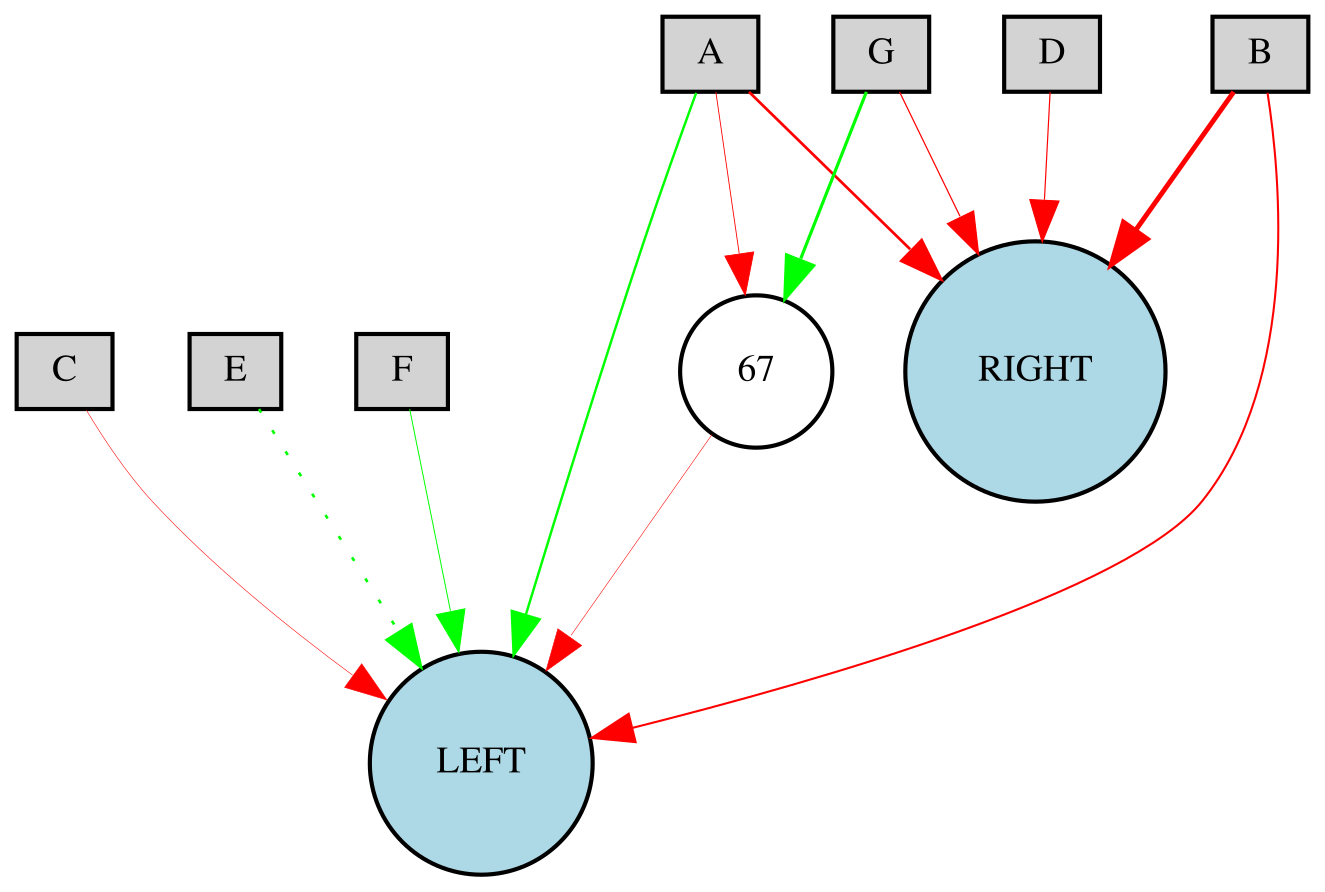
\includegraphics[scale=0.4]{include/images/thymio_network_73.PNG} \\
$$Genome \;  \; 379$$  & $$Genome \;  \; 78$$  & $Genome \;  \; 73$  \\
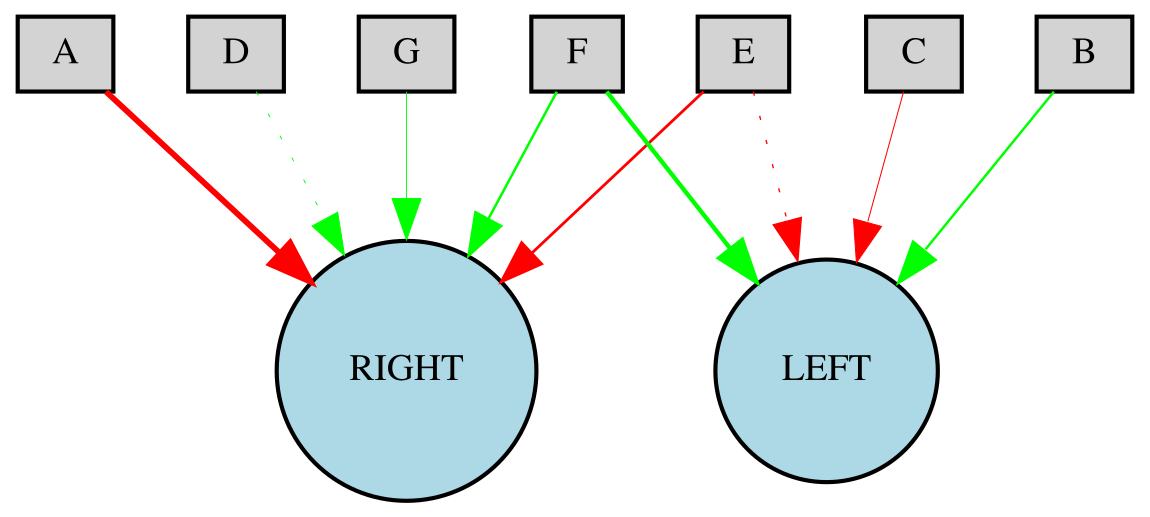
\includegraphics[scale=0.4]{include/images/thymio_network_343.PNG} & 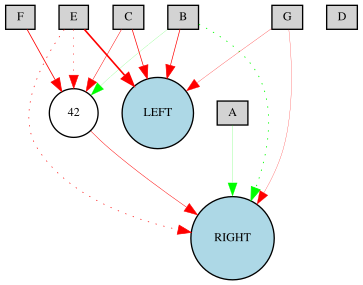
\includegraphics[scale=0.4]{include/images/thymio_network_50.PNG} & 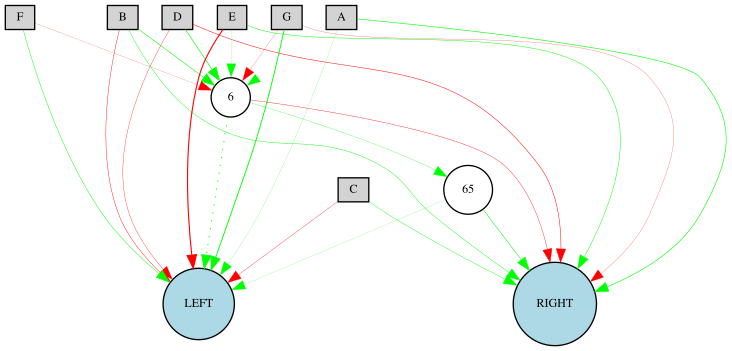
\includegraphics[scale=0.4]{include/images/thymio_network_189.PNG} \\
$Genome \;  \; 343$  & $Genome \;  \; 50$  & $Genome \;  \; 189$  \\
\end{tabular}
\caption{Evolved topology of the best controllers in reality.}
\label{fig:thymio_network_topologies} % 
\end{table}

\section{Transferability Approach}.

This series of experiments falls into the \emph{robot-in-the-loop simulation-based optimization}. Our aim is to validate the transferability approach to obstacle avoidance task based on \citep{koos2012transferability}. We assume that more transfers from simulation to reality allow to approximate the surrogate model better which could guide the evolutionary search to more transferable controllers.

\subsection{Experimenal design}

The transferability approach relies on a multi-objective formulation of the evolutionary strategy where the two main objectives are optimized with Pareto-based ranking scheme. Our implementation relies on the \citep{deb200fast} evolutionary algorithm implemented via the \emph{DEAP}\footnote{\url{https://deap.readthedocs.io/en/master/}} library. Each controller is evaluated by three objectives:

\begin{enumerate}
	\item the \emph{task-dependent fitness}\ref{eq:fitness_function}, to find controllers with obstacle avoidance behavior. 	The algorithm maximizes this objective.
	\item the corresponding \emph{simulation-to-reality disparity} (STR disparity), which is minimized, to find optimal transferable controllers.
	\item the \emph{behavioral diversity} objective, which is maximized, to find more diverse set controllers.
\end{enumerate}

\emph{STR disparity and the surrogate model}. The transferability of a given controller is evaluated by the  STR disparity measure \(D^{*}_{{c}}\), which directly quantify the behavioral disparities between any possible controller observed in simulation and in reality. The same STR disparity measure is used in our experiment as in the original implementation. Its computed as the mean square error between the corresponding trajectories between simulation and in reality during evaluation. The exact STR disparity \(D^{*}_{{c}}\) of a controller is defined as:

\begin{equation}
	D^{*}_{{c}} = \sum_{t=1}^{t_{max}} \frac{(x^{i}_{S} - x^{i}_{R})^{2}}{\bar{x_{S}}\bar{x_{R}}} + 							  \sum_{t=1}^{t_{max}} \frac{(y^{i}_{S} - y^{i}_{R})^{2}}{\bar{y_{S}}\bar{y_{R}}}
	\label{eq:The exact STR disparity measure.}
\end{equation}

Where $ S_{t_{max}} = \{{x_{S}, y_{S}} \}$  and $ R_{t_{max}} = \{ {x_{R}, y_{R}} \} $ is a set of positions extracted in simulation and reality, $ \bar{x_{S}} $ (resp. $ \bar{y_{S}}, \bar{x_{R}}, \bar{y_{R}} $) is the mean of $ x^{t_{max}}_{S} $ (resp. $ y^{t_{max}}_{S}, x^{t_{max}}_{R}, x^{t_{max}}_{R} $). The exact STR disparity measure cannot be used directly for the optimization scheme for each controller, because it would require to transfer each controller during the evaluation, therefore the approach relies on a so called \emph{surrogate model} which approximates this measure. The surrogate model is approximated by Inverse Distance Weightining interpolation method \citep{shepard1968two}. The \emph{surrogate model of the STR disparity} is defined:

\begin{equation}
	
	\[ \forall{c}\in\chi, \hat{D}_{(c)} = \frac{\sum_{c_i\in\chi_T} {D^{*}_{(c)} b_{dist}(c_{i}, c)^{-2}}}
										{\sum_{c_i\in\chi_T} {b_{dist}(c_{i}, c)^{-2} }} \]
	\label{eq:surrogate_model}
\end{equation}

Where $\chi$ is the set of all controllers in the population, $\chi_T \subset \chi$ is the set of the already transferred controllers and $D^{*}_{(c)}$ is the exact STR disparity value corresponding to each controller $c_i \in \chi_T$.

The last evaluation objective of the optmization scheme is the \emph{behavioral diversity}, which quantify the diversity of a controller from the already transfered ones. For a given controller the diversity $ diversity_{(c)}$ is:

\begin{equation}
	diversity = \min_{\forall c_i \in \chi_T } b_{dist}(c, c_i)
	\label{eq:behavioral_diversity}
\end{equation}

$b_{dist}$ is the euclidean distance between the \emph{12th} dimensional behavioral features\ref{eq:behavioral_features}.

For this approach we use a feed-forward neural network with static structure. The network is fully connected, containing 7 input neurons, 1 hidden layer with 14 neurons, and 2 motor neurons calculating the wheel speeds. The activation function is the same as in the previous experiments. In this case the genome encodes the weights of the neural network as a vector of floating point values. All genomes are bound to two genetic operators. Two point crossover is applied with probability 0.5 and a gaussian mutation with probability 0.7 mutating each attribute of the genome. The experimental configuration can be seen in table \ref{tab:moea_parameters}

\begin{table}[H]
\begin{tabular}{ll}
\hline
\textbf{}                      & \textbf{} \\ \hline
\textbf{Population Size}       & 80        \\
\textbf{Number of Generations} & 40        \\
\textbf{Simulation time}       & 40 sec    \\
\textbf{Crossover}             & 0.2       \\
\textbf{Mutation}              & 0.1       \\
\textbf{Tournament Selection}  & 3        
\end{tabular}
\caption{Parameters of the Multi-objective optmization procedure.}
\label{tab:moea_parameters}
\end{table}


\emph{Algorithm outline}. The multiobjective evolutionary strategy starts by initialzing the surrogate model of the STR disparity function by randomly selecting a $c_{(0)}$ controller among the first population. The $c_{(0)}$ controller is evaluated in simulation and then transfered to reality. The corresponding STR disparity $ D^{*}_{(c_0)}$ value, behavioral features are obtained and the surrogate model is computed/initialized. Afterwards, each generation of the algorithm follows as:

\begin{description}
	\item[1. Evaluation] of each controller
		\begin{description}
			\item[STEP 1] Computation of the task-dependent fitness, behavioral features in simulation. Respectively, aggregating the path traveled.
			\item[STEP 2] Evaluation of the approximated STR disparity (surrogate model) and behavioral diversity, based on the already transfered controllers.
		\end{description}
	\item[2. Transferability selection] 
		\begin{description}
			\item[STEP 1] Controllers with high enough diversity are selected from the current population and transferred to reality.
			\item[STEP 2] Computation of the exact STR disparity measure between the simulation and reality. Updating the surrogate model based on obtained results.
		\end{description}
	\item[3. Genetic Operators] Application of the genetic operators (crossover & mutation)
\end{description}


\emph{Complications of the implementation.} In order order to obtain controllers that transfer well from simulation to reality we tried to implement the original implementation with all its perks. Nevertheless, we have discovered/encountered the following issues:

\begin{description}
	
    \item{STR Disparity Measure}. In the initial experiments, we have defined the exact STR disparity measure as the Euclidean distance between the corresponding trajectories observed in simulation and in reality. It has been changed to the mean square error from the original implementation, which also turned out to evaluate more accurately the error between simulated and real trajectories. As it can be seen on a sample \ref{fig:trajectory_discrepancy}, the traveled discrepancies between simulation and reality computed with the Euclidean distance is \textit{1.958}, on the other hand, the discrepancy computed with the mean squared error is \textit{26.596}. This turned out to be problematic when comparing trajectories that are highly diverse, which resulted in a badly modeled surrogate model. Relying on the mean square error had the benefit of penalizing large errors more, which was appropriate to accurately model the surrogate model. 
    
    \item{Calculation of the exact Disparity Measure}. As one can assume from figure \ref{fig:trajectory_discrepancy}, it is clear that the Thymio (transferred controller in reality) is moving faster than its counterpart in simulation, based on the behavioral features, it showed that the transferred controllers average wheel speed values are much higher than in simulation, this is the result of a reality gap. In consequence with our initial constraints of measuring the disparity lead to inaccurate results of the exact disparity between simulation and reality, likewise inaccurate surrogate model. Since our implementation was concerned of taking always the N-M (or vice versa) size of [(x1,y1), (x2, y2), ...] coordinate samples both from simulation/reality, thus calculating the mean square error based on only N-M samples. It notably means that the exact str disparity measure is over-fitting, therefore not sufficient to describe the disparities. Furthermore, the collision detection was also applied for the transferred controllers, which also skewed the values. This miscalculation is depicted in figure \ref{fig:trajectory_discrepancy_wrong_measure}. To cope with these potential miscalculations, this constraint was removed and later on the entire trajectory is used to correctly calculate the exact STR disparity.
	
\end{description}

\begin{figure}[H]
    \centering
    \begin{subfigure}[b]{0.8\textwidth}
    	\centering
        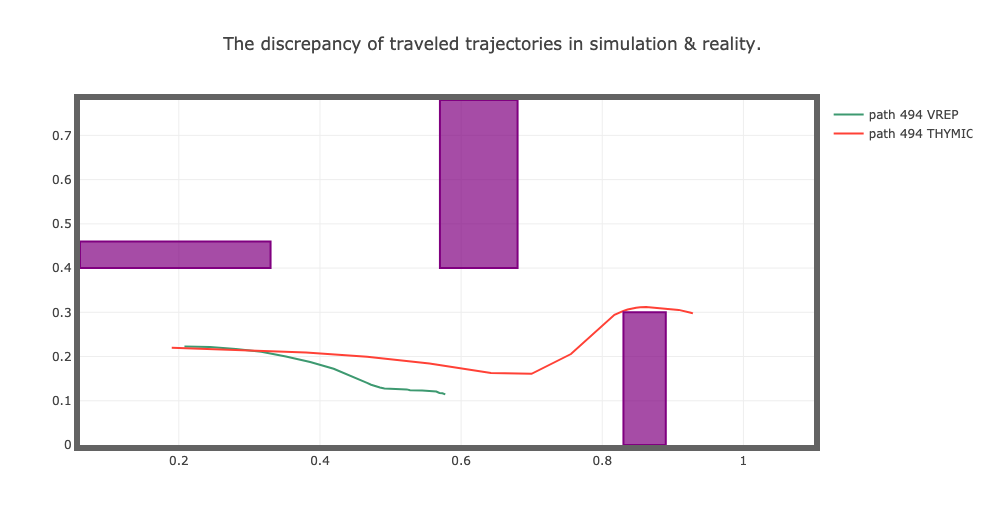
\includegraphics[width=5cm]{include/images/trajectory_discrepancy.PNG}
        \caption{The discrepancy of traveled trajectories in simulation and reality.}
        \label{fig:trajectory_discrepancy}
    \end{subfigure}
    \begin{subfigure}[b]{0.8\textwidth}
    	\centering
        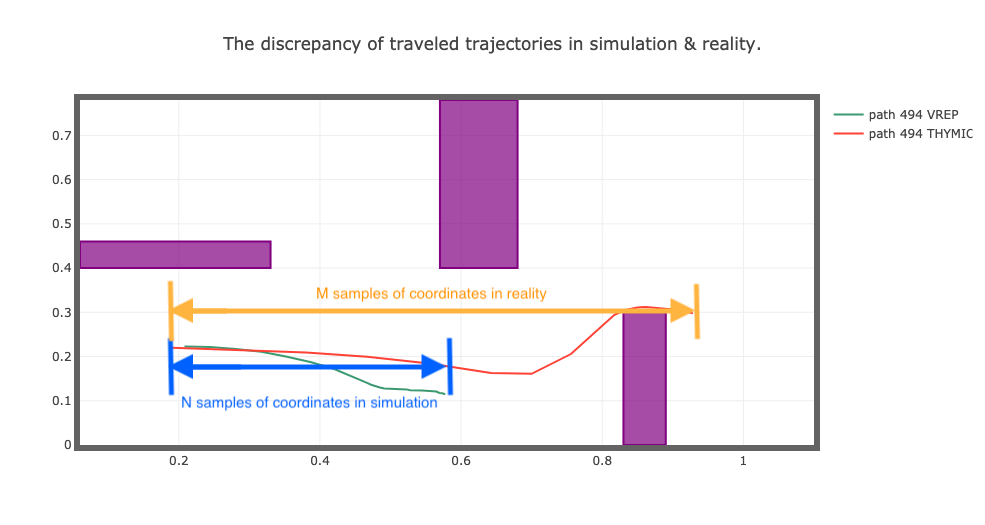
\includegraphics[width=5cm]{include/images/trajectory_discrepancy_wrong_measure.PNG}
        \caption{Potential miscalculations of the exact STR Disparity.}
        \label{fig:trajectory_discrepancy_wrong_measure}
    \end{subfigure}
    % \caption{Reality-based simulation results I.}
	\label{fig:real_based_resultsI}
\end{figure}



\subsection{Results}




\section{Discussion}




\chapter{Conclusion}

In this thesis, we have built an automated robotic platform with features that enhances the ability to test and validate evolutionary optimization procedures both in simulation and in reality, run the entire optimization process on the physical robot without human intervention. Furthermore, to perform a completely autonomous co-evolution of controllers which can take place in simulation and in reality too. This proved to be useful for the robot-in-the-loop simulation-based optimization approaches, especially for the \emph{Transferability approach}. In which we have been able to seamlessly conduct many transfer experiments during the optimization procedure. The mixed reality module of the system enabled to minimize the evaluation time of the overall experiments.

We've spent a significant portion of the thesis into the construction of the automated robotic platform. Combining the various software frameworks to manage the reality-based optimization and co-evolution of the simulation tools. Various tests and modifications have been performed to validate the robustness and functionality of the platform. Ultimately the automated robotic platform is a contribution towards the application of different reality-gap methods for passing the reality gap.

Furthermore, in this thesis, we have addressed the reality gap problem by performing simulation-based, reality-based and robot-in-the-loop optimization procedures on an obstacle avoidance task. We concluded benchmark experiments in simulation and reality using the NEAT algorithm. These benchmarks have been used as a baseline to compare the results with the transferability approach. This approach has been reproduced based on the original implementation \citep{koos2012transferability}. We have discovered that many things can go wrong within this approach, but all in all we were able to confirm our hypothesis. Better results were achieved by the \emph{Transferability} approach when more transfers were conducted on the physical robot. Based on the successful results, we have evolved controllers with no transferability issues. Thus we can come to the conclusion that \emph{transferability} approach is indeed the relevant technique to cross the reality gap with a more accurate surrogate model.

The whole project is hosted on github \footnote{https://github.com/richban/behavioral.neuroevolution}.




\nocite{*} % includes ALL documents in the bibliographic database whether or not cited in the text
\bibliography{bibliography/bibliography}
\bibliographystyle{apacite}

\end{document}